	\newgeometry{textwidth=16cm}
\chapter[longue portee]{Systèmes en interaction à longue portée - De la nécessité des approches DFT}
\minitoc
\restoregeometry

\newpage

\section*{Introduction}
\markright{INTRODUCTION}{}

Un des challenges qui nous ont été proposés initialement par les expérimentateurs a été celui de la caractérisation des molécules et de leurs interactions au sein des mélanges d’asphaltènes. Comme nous l’avons rappelé dans le chapitre I, très peu d’informations sont connues à ce sujet à l’heure actuelle. Aucune technique de caractérisation, quelle soit physique ou chimique, n’est véritablement à même de répondre précisément à cette question. J. Shaw a proposé (ref), bien avant les autres acteurs du domaine, que ces systèmes « associés » pouvaient être caractérisés à l’aide des spectroscopies Infra-Rouge et Raman, en utilisant notamment la technique de la photo-acoustique, dans le but d’accéder aux informations spectrales de très bas nombres d’ondes (zone spectrale suspectée de contenir la signature des modes de libration associés aux interactions intermoléculaires). Au-delà des difficultés inhérentes au manque d’informations, aussi bien quant à la nature des molécules et des familles qui constituent ces mélanges complexes que concernant le rôle des hétéroéléments, une autre des difficultés qui s’est imposée à nous concernait le traitement quantique vibrationnel de systèmes de grande dimension et, qui plus est, en interaction. En admettant même que les deux problèmes vibrationnels majeurs, i.e. la détermination de la SEP et la résolution de l’équation vibrationnelle de Schr\"{o}dinger, soient absents et indépendants de la dimension du problème (ce qui n’a bien entendu aucun sens, comme nous l’avons montré dans le chapitre II), la prise en compte dans nos modèles quantiques des interactions est à elle seule un des problèmes majeur qu’il nous a fallu intégrer dès le départ, sous peine de ne pouvoir fournir aux expérimentateurs des données suffisamment fiables pour rendre compte des observations spectroscopiques. 

Ainsi, pour ce qui concerne le traitement quantique des interactions intermoléculaires, qui fait l’objet principal de ce chapitre, il est important de rappeler que notre travail ne se situe pas dans un contexte de développement méthodologique mais plutôt dans un contexte de recherche des stratégies calculatoires les plus adaptées pour traiter de problèmes vibrationnels concernant des systèmes chimiques en interactions, de grandes dimensions, qu’une méthode fortement corrélée ne permet pas encore d’atteindre \footnote{malgré les progrès particulièrement significatifs réalisés au cours de ces dernières années, tels que l’emploi de bases cc-pVXZ-F12 (X=D,T,Q) développées pour l’utilisation de méthodes explicitement corrélées (citons notamment les bases dédiées à la résolution des approximations d'identité RI (en anglais « Resolution Identity »)), des approximations d'ajustement de la densité DF (en anglais « Density Fitting ») pour le calcul d’intégrales, la non-linéarité des facteurs de corrélation, etc.}. L’utilisation de la DFT s’est donc naturellement imposée à nous.

Force est de constater les progrès réalisés depuis une décennie dans la description du formalisme de la théorie de la fonctionnelle de la densité, qui rendent son utilisation quasi-inéluctable. Bien loin des effets de mode, on constate les réussites frappantes de la DFT dans la description de propriétés telles que les liaisons, les structures, la cohésion aussi bien au niveau moléculaire que dans les solides. Néanmoins, il est des domaines dans lesquels les progrès sont encore lents et ou les méthodes sont encore mises en défaut : tels que le traitement des atomes lourds, les systèmes possédant des électrons fortement corrélés, le traitement crucial en réactivité des états multi déterminantaux, le problème de la correction de la self-itération et, bien entendu, le problème qui nous occupe directement de la description des forces de dispersion. Cette dernière problématique n’est pas récente puisque elle émerge des premiers travaux de Gordon et Kim (R. G. Gordon and Y. S. Kim, J. Chem. Phys. 56, 3122 (1972)) en 1972. Elle s’avère particulièrement prégnante pour l’étude des systèmes fortement liés (tels certains oxides métalliques) et dans les cas où les forces de van der Waals sont prédominantes (matière molle, complexes de van der Waals, biomolécules et autres matériaux lamellaires). L’origine de ce problème est désormais clairement identifiée i.e. les effets de corrélation électronique des forces de dispersion sont purement non locaux et, en aucun cas, une approximation locale ou semi-locale ne pourra en rendre compte. Si la fonctionnelle d’échange-corrélation exacte pouvait être connue, il serait cependant possible de répondre à la question posée par la description des forces de vdW dans le formalisme KS. Cela fait plus d’une décennie que la recherche dans ce domaine est extrêmement active. L’idée qui prévaut aujourd’hui est celle de développer des méthodes ayant les moyens, à un moindre coût computationnel, d’incorporer des corrections au formalisme KS sans perdre de vue les avantages de la DFT aussi bien au niveau moléculaire que dans le calcul en conditions périodiques. 

Rappelons que l’utilisation pratique de la DFT dans son formalisme KS repose sur l’approximation de la fonctionnelle d’échange-corrélation. L’approximation originelle i.e. l’Approximation de Densité Locale (LDA pour l’anglais Local Density Approximation), s’est révélée étonnamment efficace et difficile à améliorer de manière systématique. Il a été montré que la LDA, étant locale par construction, est particulièrement adaptée pour décrire les corrélations à très courte-portée inter-électronique, mais échoue à décrire quantitativement les corrélations à longue-portée électronique. Ceci reste vrai avec la plupart des améliorations post-LDA classiques (que nous n’aborderons pas dans ce travail), qui demeurent par design des approximations de nature locale. Différentes solutions existent désormais pour traiter ce problème. Citons par exemple sans aucune volonté d’exhaustivité, avec différents niveaux d’empirisme, les travaux autour de paramétrisations spécifiques de nouvelles fonctionnelles GGA ou méta-GGA (Truhlar et al., J. Chem. Phys., 125, 194101 (2006)), les travaux de type DFT+D incluant des corrections de dispersion de Grimme pour ne citer que le plus connu (Grimme, J. Comput. Chem., 27, 1787 (2006), J. Chem. Phys, 132, 154104 (2010), les travaux de type Symetrized Adapted Perturbation Theory SAPT ou SAPT(DFT) même si ces derniers ne s’attachent plus tout à fait à la recherche d’une fonctionnelle d’échange-corrélation, et les travaux qui vont finalement s’atteler à donner une forme explicite de la fonctionnelle d’échange-corrélation (vdW-DF non-local vdW correlation functional Michaelides et al., J. Chem. Phys., 137, 120901 (2012) ; Hutter et al., J. Chem. Phys., 138, 204103 (2013)) en recherchant son caractère non-local (notamment à travers de l’application du théorème de fluctuation-dissipation combiné à la connexion adiabatique – telle que les méthodes AC-FDT, DRSLL M. Dion, H. Rydberg, E. Schröder, D. C. Langreth, and B. I. Lundqvist, Phys. Rev. Lett. 92, 246401 (2004); 95, 109902 (2005) et Bayesian error estimation functional BEEF Jacobsen et al. Phys. Rev. B, 85, 235149 (2012)). Parmi ces dernières solutions non-empiriques, on peut citer notamment les modèles d’Anderssson-Langreth-Lundqvist (ALL) ou ceux de type Random Phase Approximation (RPA) qui ont très récemment fait l’objet d’études approfondies de la part, par exemple, de S. Lebègue et coll (S. Lebègue, J. Harl, Tim Gould, J. G. Ángyán, G. Kresse, and J. F. Dobson Phys. Rev. Lett. 105, 196401 (2010)).\\

 
Pour résumer, on peut rappeler que d’un point de vue théorique l’énergie d’interaction intermoléculaire est une observable que l’on peut soit calculer directement (à l’aide d’une approche globale de type ‘supermolécule’) soit chercher à interpréter par différentes décompositions auxquelles on souhaite adjoindre, dans la mesure du possible, un sens physique. Nous avons fait le choix arbitraire, dans la première partie de ce chapitre, de présenter les termes d’interaction à partir de la théorie de perturbation développée jusqu’au second ordre. Cette présentation nous semblait justifiée par le fait qu’une fois les hypothèses de travail définies et une fois les fonctions de réponses nécessaires au calcul des termes d’interactions établies, la présentation des approches méthodologiques les plus avancées dans ce domaine s’en trouvait facilité. De plus, parce qu’il est désormais acquis qu’un tel traitement conduit généralement à une mauvaise convergence de la série de perturbation, nous profiterons de cette présentation pour introduire l’approche SAPT (Symmetrized Adapted Perturbation théorie) qui corrige ces divergences et qui est considérée aujourd’hui comme l’une des plus précise pour le calcul des énergie d’interactions intermoléculaires. 
De façon formelle toutes les approches présentées dans cette première partie n’imposent pas l’utilisation des approches de la DFT. Néanmoins, de façon pratique, de part la dimension et la diversité des systèmes que l’on a à étudier, l’emploi des approches DFT est inéluctable. Ainsi, après avoir donné dans la seconde partie de ce chapitre quelques rappels sur les fondements théorique de la méthodologie DFT, nous présenterons la notion de fonctionnelle hybride puis présenterons le principe des approches employées dans ce travail qui ajoutent ad hoc des fonctions semi-empiriques rendant compte des effets de dispersion à un calcul KS usuel.\\












%%%%%%%%%%%%%%%%%%%%%%%%%%%%%%%%%%%%%%%%%%%%%%
%%%%%%%%%%%%%%%%%%%%%%%%%%%%%%%%%%%%%%%%%%%%%%
%%%%%%%%%%%%%%%%%%%%%%%%%%%%%%%%%%%%%%%%%%%%%%
%%%%%%%%%%%%%%%%%%%%%%%%%%%%%%%%%%%%%%%%%%%%%%
\section[Théorie des perturbations]{Théorie des perturbations}
%%%%%%%%%%%%%%%%%%%%%%%%%%%%%%%%%%%%%%%%%%%%%%
%%%%%%%%%%%%%%%%%%%%%%%%%%%%%%%%%%%%%%%%%%%%%%
%%%%%%%%%%%%%%%%%%%%%%%%%%%%%%%%%%%%%%%%%%%%%%
%%%%%%%%%%%%%%%%%%%%%%%%%%%%%%%%%%%%%%%%%%%%%%

Au delà des liaisons hydrogènes et des interactions de nature électrostatique (\textit{e.g.} charge- charge, charge- dipôle, dipôle- dipôle), l’autre interaction non covalente la plus étudiée à l’heure actuelle est probablement celle impliquant les systèmes aromatiques \cite{grimme2008special}. Ces interactions dénommées ‘pi-stacking’ entre cycles aromatiques (peut être à mauvais escient (Chelsea R. Martinez and Brent L. Iverson Chem Science 2012,3, 2191-2201) sont notamment considérées comme responsables de la stabilité d’un très grand nombre de structures remarquables \cite{mcgaughey1998pi} dont celles qui préfigurent certainement la structures des asplhaltènes. L’étude expérimentale de ces interactions présente encore un défi car il est généralement compliqué de séparer les interactions $\pi$-stacking des interactions secondaires ou des effets de l’environnement. A cause de ces difficultés expérimentales, les études en chimique computationnelle apparaissent comme une alternative de choix pour comprendre la nature fondamentale des ces interactions non covalentes, ainsi que leur influence sur les systèmes chimiques étudiés. Nous encourageons le lecteur à se reporter au travail de revue Martinez et Iverson concernant ce sujet, revue dans laquelle sont recensés les principales définitions et les principaux modèles employés pour décrire ces interactions particulières.
Le graal pour les expérimentateurs comme pour les théoriciens serait d’arriver, \textit{in fine}, à pouvoir caractériser séparément la contribution de chacune des ces interactions non-covalentes et d’en prévoir leur rôle et leur intensité.\\

Quoi qu’il en soit, nous savons désormais que l’énergie d'interaction intermoléculaire d'un ensemble de molécules se situe généralement entre 1 et 20 kcal/mol selon le nombre et le type de molécules impliquées. Cependant, l'énergie d'une liaison chimique covalente se mesure entre 100 et 300 kcal/mol, ce qui est d’un autre ordre de grandeur. De même, la portée d’une liaison chimique dépasse rarement quelques Angströms tandis que les interactions intermoléculaires s'étendent théoriquement jusqu'à l'infini (électrostatique) et de manière pratique entre 2 et 10 Angströms selon la taille et la nature du système.\\

D’un point de vue théorique l’énergie d’interaction intermoléculaire est une observable qu’on peut interpréter par différentes décompositions auxquelles on souhaite adjoindre, dans la mesure du possible, un sens physique. Buckingham \cite{buckingham1967permanent} proposait déjà en 1967 une décomposition de l’énergie d’interaction intermoléculaire en quatre grandes contributions : l’électrostatique $E_{elec}$, l’induction $E_{ind}$, l’echange-repulsion $E_{rep}$, et la dispersion $E_{disp}$.\\

\begin{equation}
\Delta E = E_{elec} + E_{ind} + E_{rep} + E_{disp}
\end{equation} 

L’interaction électrostatique est l’ensemble des interactions coulombiennes existant entre deux densités de charges isolées. Elle est additive et peut être répulsive ou attractive selon l’orientation relative des molécules. Elle constitue la plus grande partie de l’interaction intermoléculaire. 
 
L’énergie d’induction quand à elle due à la déformation de la densité électronique d’un atome ou d’une molécule par l’effet du champs électrique d’une molécule voisine. Cette énergie est non additive et toujours attractive.\\

Ces deux contributions sont très bien définies en physique classique, contrairement à la dispersion et à l’échange, qui sont liés à des effets quantiques.\\

La répulsion vient du principe de Pauli, qui stipule que deux électrons ne peuvent pas occuper le même spin au sein d’une même orbitale. C’est une interaction toujours répulsive et qui apparaît seulement à courte distance.\\

Finalement la dispersion n’a pas d’équivalent classique car c’est une interaction qui est liée à la corrélation électronique de deux densités de charge en interaction (fluctuation quantique des distributions de charges). Elle est attractive et existe dans tous les complexes.\\

Il y a, de façon pratique, deux manières différentes de calculer une énergie d’interaction intermoléculaire. L’une est la méthode appelée en « supermolécules », et l’autre est la méthode consistant en la construction de l’interaction intermoléculaire à partir de la connaissance des réponses des fonctions d’onde des monomères séparés (au sein du dimère) soumis à l’action de perturbations externes.\\

%%%%%%%%%%%%%%%%%%%%%%%%%%%%%%%%%%%%%%%%%%%%%%
%%%%%%%%%%%%%%%%%%%%%%%%%%%%%%%%%%%%%%%%%%%%%%
%%%%%%%%%%%%%%%%%%%%%%%%%%%%%%%%%%%%%%%%%%%%%%
\subsection{l’approche en « supermolécules »}
%%%%%%%%%%%%%%%%%%%%%%%%%%%%%%%%%%%%%%%%%%%%%%
%%%%%%%%%%%%%%%%%%%%%%%%%%%%%%%%%%%%%%%%%%%%%%
%%%%%%%%%%%%%%%%%%%%%%%%%%%%%%%%%%%%%%%%%%%%%%

Dans la méthode supermoléculaire l’énergie d’interaction intermoléculaire est obtenue comme la différence entre l’énergie totale du dimère et la somme de l’énergie total de chaque monomère.

\begin{equation}
\Delta E = E_{AB} - E_{A} - E_{B} \label{eq2}
\end{equation}

A et B représentent les monomères et AB le dimère. Dans ce cas là, une erreur subtile peut se produire autour de l’énergie d’interaction. Cette erreur est connue sous le nom de Basis Set Superposition Error (BSSE) \cite{sherrill2010counterpoise}. Si nous calculons les deux monomères dans leurs bases spécifiques, et ensuite un dimère dans l’ensemble des fonctions de base des monomères, nous pourrons utiliser les orbitales virtuelles d’un monomère pour agrandir la base disponible pour la distribution de charge de l’autre monomère et vice versa. Le résultat est donc une augmentation de la qualité de la base pour le dimère vis-à-vis des monomères, et par conséquent une surestimation de l’énergie de l’interaction. Pour corriger l’erreur de BSSE, une méthode possible est de travailler dans une base complète ou saturée pour les monomères et le dimère. Une autre méthode est de calculer l’énergie des monomères dans la base du dimère, ce qui est le plus fréquemment utilisé sous le nom de counterpoise grace a Boys et Bernardi \cite{boys1970calculation}. Cette correction entraîne que pour chaque distance intermoléculaire considérée il est nécessaire de calculer l’énergie totale du dimère et des monomères.\\

L’énergie sans correction donnée pour l’équation \ref{eq2}  peut-être modifiée pour l'estimation de la quantité pour laquelle le monomère A est stabilisé artificiellement pour la base supplémentaire du monomère B et vice versa, avec la relation suivante:

\begin{equation}
E_{BASE}(A) = E_{A}^{AB}(A) - E_{A}^{A}(A)
\end{equation}

\begin{equation}
E_{BSSE}(B) = E_{B}^{AB}(B) - E_{B}^{B}(B)
\end{equation}

où l'exposant désigne la base utilisée, l'indice désigne la géométrie et le symbole entre parenthèses est le système chimique considéré.
L'énergie d'interaction corrigée est donc donnée par l'expression suivante :

\begin{equation}
E^{CP} = E_{A-B}^{A-B}(A-B) - E_{A}^{A-B}(A) - E_{B}^{A-B}(B)
\end{equation}

Dans ces conditions, les électrons de chaque fragment du système bénéficient de la base d'orbitales des autres fragments. La correction de la BSSE est par définition la différence entre l'énergie d'interaction non corrigée et l'énergie corrigée :

\begin{equation}
\Delta E^{CP} = E - E^{CP} = (E_{A-B}^{A-B}(A-B) - E_{A}^{A}(A) - E_{B}^{B}(B)) - (E_{A-B}^{A-B}(A-B) - E_{A}^{A-B}(A) - E_{B}^{A-B}(B))
\end{equation}

\begin{equation}
\Delta E^{CP} =  E_{A}^{A-B}(A) - E_{B}^{A-B}(B) - E_{A}^{A}(A) - E_{B}^{B}(B)
\end{equation}

Les bases ayant une extension spatiale finie, cette erreur est d'autant moins importante que les molécules sont éloignées les une des autres. La BSSE étant nulle dans la limite des bases infinies. En pratique le calcul de la BSSE doit donc être effectué pour chaque conformation d’énergie minimale déterminée pour chaque distance intermoléculaire qui sépare les espèces A et B. Plus la base est petite plus cette erreur est importante. Dans la limite d’une base complète la BSSE s’annule.
Les calculs HF et KS souffrent moins des effets de la BSSE (J. Garza, J.-Z. Ramírez, and R. Vargas, J. Phys. Chem. A 109, 643 (2005))
qui sont plus marqués dans les calculs post-HF (MPn, CCSD(T)), du fait en particulier du traitement de l’espace des virtuels nécessaire pour ces approches.\\


Malheureusement, le calcul direct d’une énergie d’interaction par la méthode « supermolécules » est extrêmement coûteux et il ne donne jamais aucune information sur la nature des interactions mises en jeu.\\

%%%%%%%%%%%%%%%%%%%%%%%%%%%%%%%%%%%%%%%%%%%%%%
%%%%%%%%%%%%%%%%%%%%%%%%%%%%%%%%%%%%%%%%%%%%%%
%%%%%%%%%%%%%%%%%%%%%%%%%%%%%%%%%%%%%%%%%%%%%%
\subsection{Détermination théorique des coefficients du développement multipolaire de l’énergie interaction à grande distance : Potentiel électrostatique}
%%%%%%%%%%%%%%%%%%%%%%%%%%%%%%%%%%%%%%%%%%%%%%
%%%%%%%%%%%%%%%%%%%%%%%%%%%%%%%%%%%%%%%%%%%%%%
%%%%%%%%%%%%%%%%%%%%%%%%%%%%%%%%%%%%%%%%%%%%%%


La première théorie qui, en mécanique quantique, a été proposé pour déterminer la nature des interactions intermoléculaire a été développée dès 1927 par Wang \cite{wang1927mutual}  puis reprise et très largement étendue à partir de 1930 par London et al \cite{london1930z}. Nous avons fait le choix, dans les paragraphes qui vont suivre, de ne mener le recensement des termes d’interactions introduits par London que jusqu’aux plus bas ordres de perturbation i.e. les interactions de distorsion et de dispersion que l’on peut relier aux propriétés électroniques des fragments interagissant, trouvent leurs origines dans des effets du second ordre. Les choix du modèle et de la troncature sont eux aussi totalement arbitraires puisqu’il existe aujourd’hui d’autres modèles tels ceux de  Kitaura et Morouma \cite{morokuma1977molecules} et de Stevens et Fink \cite{stevens1987frozen} pour ne citer qu’eux. Le modèle perturbatif est celui qui, à notre avis, permet la meilleur compréhension de la physique qui se cache derrière les forces de dispersion et de rendre compte des coefficients ‘dits’ de van der Waals ainsi que des fonctions de réponses qui leur sont associées tels que les polarisabilités multipolaires elles même reliées aux fonctions spectrales telles que les forces d’oscillateurs et les énergies d’excitations (ref). Enfin, le choix de présenter les termes d’interaction à partir de la théorie de perturbation nous semblait aussi justifié par le fait qu’une fois les hypothèses de travail définies et une fois les fonctions de réponses établies, la présentation des approches de type SAPT (Symetrized Adaptative Perturbation Theory) et des méthodes basées sur la détermination des fonctions semi-empiriques devant rendre compte des effets de dispersion s’en trouvent facilitées et justifiées.


Dans ce paragraphe consacré aux interactions à longues distances, nous allons donner les expressions générales du hamiltonien d'interaction, et établir à l'aide de la méthode de perturbation les équations du problème.\\ 

Soient deux systèmes $a$ et $b$ qui à l'état isolé sont susceptibles de se trouver dans les états $\phi_{0}^{a}$ ... $\phi_{p}^{a}$ et $\phi_{0}^{b}$ ... $\phi_{q}^{b}$ fonctions propres des hamiltoniens $H_{0}(a)$ et $H_{0}(b)$ correspondants aux énergies $E_{0}^{a}$ ... $E_{p}^{a}$ et $E_{0}^{b}$ ... $E_{q}^{b}$. Lorsque ces deux systèmes interagissent, le hamiltonien du système global s'écrit : 

\begin{equation}
H = H_{0}(a) + H_{0}(b) + H'
\end{equation}

Le système crée au niveau de $b$ un potentiel électrostatique $\Phi_{Kb}$ avec lequel les charges de $a$ interagissent, donnant naissance à une énergie d'interaction (et réciproquement au niveau du système $b$).

%%%%%%%%%%%%%%%%%%%%%%%%%%%%%%%%%%%%%%%%%%%%%%
%%%%%%%%%%%%%%%%%%%%%%%%%%%%%%%%%%%%%%%%%%%%%%
\subsubsection{Hamiltonien à l'ordre zéro pour le système [$a-b$]}
%%%%%%%%%%%%%%%%%%%%%%%%%%%%%%%%%%%%%%%%%%%%%%
%%%%%%%%%%%%%%%%%%%%%%%%%%%%%%%%%%%%%%%%%%%%%%

A distance suffisamment grande pour que les distributions de charges liées aux systèmes $a$ et $b$ ne se recouvrent pas (on considère que celles-ci sont séparées), le hamiltonien à l'ordre zéro qui représente le système [$a-b$] est simplement la somme des hamiltoniens propres dus système $a$ et du système $b$. D'où : 

\begin{equation}
H_{0} = H_{0}(a) + H_{0}(b) \label{1.2}
\end{equation}

avec : 

\begin{equation}
H_{0}(a) = -\frac{1}{2} \sum_{k_{a}=1}^{n_{a}} \triangledown^{2} k_{a} - \sum_{k_{a}=1}^{n_{a}} \frac{Z_{a}}{rk_{a}} + \sum_{k'_{a}>k_{a}} \frac{1}{rk_{a},k'_{a}} + H_{l.s}(a)  \label{1.3}
\end{equation}

Où $\triangledown_{k_{a}}$, $Z_{a}$, $r_{k_{a}}$ et $rk_{a},k'_{a}$ représentent respectivement l'opérateur énergie cinétique, la charge du noyau de $a$, les distances noyau- électron $k_{a}$ et électron $k_{a}$- électron $k'_{a}$. L'expression de $H_{0}(b)$ se déduit facilement de celle de $H_{0}(a)$ en remplaçant les coordonnées des $n_{a}$ électrons du système $a$ par les $n_{b}$ électrons du système $b$. $H_{l.s}(a)= \sum_{k_{a}=1}^{n_{a}} \zeta_{k_{a}} \widehat{l_{k_{a}}} \widehat{S_{k_{a}}}$ est le hamiltonien de spin-orbite de l'atome $a$, $\widehat{l_{k_{a}}}$ et $\widehat{S_{k_{a}}}$ sont les operateurs moment orbital et moment de spin de l'électron $k_{a}$, et $\zeta_{k_{a}}$ une constante de couplage spin orbite pour le même électron.

%%%%%%%%%%%%%%%%%%%%%%%%%%%%%%%%%%%%%%%%%%%%%%
%%%%%%%%%%%%%%%%%%%%%%%%%%%%%%%%%%%%%%%%%%%%%%
%%%%%%%%%%%%%%%%%%%%%%%%%%%%%%%%%%%%%%%%%%%%%%
\subsection{Détermination théorique des coefficients du développement multipolaire de l’énergie interaction à grande distance : Potentiel électrostatique}
%%%%%%%%%%%%%%%%%%%%%%%%%%%%%%%%%%%%%%%%%%%%%%
%%%%%%%%%%%%%%%%%%%%%%%%%%%%%%%%%%%%%%%%%%%%%%
%%%%%%%%%%%%%%%%%%%%%%%%%%%%%%%%%%%%%%%%%%%%%%


La première théorie qui, en mécanique quantique, a été proposé pour déterminer la nature des interactions intermoléculaire a été développée dès 1927 par Wang \cite{wang1927mutual}  puis reprise et très largement étendue à partir de 1930 par London et al \cite{london1930z}. Nous avons fait le choix, dans les paragraphes qui vont suivre, de ne mener le recensement des termes d’interactions introduits par London que jusqu’aux plus bas ordres de perturbation i.e. les interactions de distorsion et de dispersion que l’on peut relier aux propriétés électroniques des fragments interagissant, trouvent leurs origines dans des effets du second ordre. Les choix du modèle et de la troncature sont eux aussi totalement arbitraires puisqu’il existe aujourd’hui d’autres modèles tels ceux de  Kitaura et Morouma \cite{morokuma1977molecules} et de Stevens et Fink \cite{stevens1987frozen} pour ne citer qu’eux. Le modèle perturbatif est celui qui, à notre avis, permet la meilleur compréhension de la physique qui se cache derrière les forces de dispersion et de rendre compte des coefficients ‘dits’ de van der Waals ainsi que des fonctions de réponses qui leur sont associées tels que les polarisabilités multipolaires elles même reliées aux fonctions spectrales telles que les forces d’oscillateurs et les énergies d’excitations (ref). Enfin, le choix de présenter les termes d’interaction à partir de la théorie de perturbation nous semblait aussi justifié par le fait qu’une fois les hypothèses de travail définies et une fois les fonctions de réponses établies, la présentation des approches de type SAPT (Symetrized Adaptative Perturbation Theory) et des méthodes basées sur la détermination des fonctions semi-empiriques devant rendre compte des effets de dispersion s’en trouvent facilitées et justifiées.


Dans ce paragraphe consacré aux interactions à longues distances, nous allons donner les expressions générales du hamiltonien d'interaction, et établir à l'aide de la méthode de perturbation les équations du problème.\\ 

Soient deux systèmes $a$ et $b$ qui à l'état isolé sont susceptibles de se trouver dans les états $\phi_{0}^{a}$ ... $\phi_{p}^{a}$ et $\phi_{0}^{b}$ ... $\phi_{q}^{b}$ fonctions propres des hamiltoniens $H_{0}(a)$ et $H_{0}(b)$ correspondants aux énergies $E_{0}^{a}$ ... $E_{p}^{a}$ et $E_{0}^{b}$ ... $E_{q}^{b}$. Lorsque ces deux systèmes interagissent, le hamiltonien du système global s'écrit : 

\begin{equation}
H = H_{0}(a) + H_{0}(b) + H'
\end{equation}

Le système crée au niveau de $b$ un potentiel électrostatique $\Phi_{Kb}$ avec lequel les charges de $a$ interagissent, donnant naissance à une énergie d'interaction (et réciproquement au niveau du système $b$).

%%%%%%%%%%%%%%%%%%%%%%%%%%%%%%%%%%%%%%%%%%%%%%
%%%%%%%%%%%%%%%%%%%%%%%%%%%%%%%%%%%%%%%%%%%%%%
\subsubsection{Hamiltonien à l'ordre zéro pour le système [$a-b$]}
%%%%%%%%%%%%%%%%%%%%%%%%%%%%%%%%%%%%%%%%%%%%%%
%%%%%%%%%%%%%%%%%%%%%%%%%%%%%%%%%%%%%%%%%%%%%%

A distance suffisamment grande pour que les distributions de charges liées aux systèmes $a$ et $b$ ne se recouvrent pas (on considère que celles-ci sont séparées), le hamiltonien à l'ordre zéro qui représente le système [$a-b$] est simplement la somme des hamiltoniens propres dus système $a$ et du système $b$. D'où : 

\begin{equation}
H_{0} = H_{0}(a) + H_{0}(b) \label{1.2}
\end{equation}

avec : 

\begin{equation}
H_{0}(a) = -\frac{1}{2} \sum_{k_{a}=1}^{n_{a}} \triangledown^{2} k_{a} - \sum_{k_{a}=1}^{n_{a}} \frac{Z_{a}}{rk_{a}} + \sum_{k'_{a}>k_{a}} \frac{1}{rk_{a},k'_{a}} + H_{l.s}(a)  \label{1.3}
\end{equation}

Où $\triangledown_{k_{a}}$, $Z_{a}$, $r_{k_{a}}$ et $rk_{a},k'_{a}$ représentent respectivement l'opérateur énergie cinétique, la charge du noyau de $a$, les distances noyau- électron $k_{a}$ et électron $k_{a}$- électron $k'_{a}$. L'expression de $H_{0}(b)$ se déduit facilement de celle de $H_{0}(a)$ en remplaçant les coordonnées des $n_{a}$ électrons du système $a$ par les $n_{b}$ électrons du système $b$. $H_{l.s}(a)= \sum_{k_{a}=1}^{n_{a}} \zeta_{k_{a}} \widehat{l_{k_{a}}} \widehat{S_{k_{a}}}$ est le hamiltonien de spin-orbite de l'atome $a$, $\widehat{l_{k_{a}}}$ et $\widehat{S_{k_{a}}}$ sont les operateurs moment orbital et moment de spin de l'électron $k_{a}$, et $\zeta_{k_{a}}$ une constante de couplage spin orbite pour le même électron.


%%%%%%%%%%%%%%%%%%%%%%%%%%%%%%%%%%%%%%%%%%%%%%
%%%%%%%%%%%%%%%%%%%%%%%%%%%%%%%%%%%%%%%%%%%%%%
\subsubsection{Fonction d'onde moléculaire à l'ordre zéro}
%%%%%%%%%%%%%%%%%%%%%%%%%%%%%%%%%%%%%%%%%%%%%%
%%%%%%%%%%%%%%%%%%%%%%%%%%%%%%%%%%%%%%%%%%%%%%

La structure électronique d'un système moléculaire et les propriétés qui en découlent peuvent être déterminées à partir de la résolution de l'équation de Schr\"{o}dinger. Pour un système constitue de $N$ électrons se déplaçant dans le champs électrostatique créé par les noyaux, cette équation s'écrit : $H\Psi = E\Psi$. La résolution de l'équation intégro-différentielle de Schr\"{o}dinger aux états stationnaires pour les systèmes pluriélectroniques n'est pas envisageable sans approximations. Les fonctions propres du hamiltonien $H$ décrivent les états du systèmes dont l'énergie est égale à la valeur propre correspondante. De l'expression \ref{1.2} du hamiltonien non perturbé, une expression de la fonction d'onde $\Psi_{00}$ décrivant l'interaction entre deux atomes $a$ et $b$ pris dans leur état fondamental peut être : 

\begin{equation}
\Psi_{00} = \phi_{0}^{a} \cdot \phi_{0}^{b}
\end{equation}

Produit non antisymétrisé des fonctions d'ondes $\phi_{0}^{a}$ et $\phi_{0}^{b}$ des systèmes $a$ et $b$ non perturbés. En toute rigueur, le simple produit des fonctions $\phi_{0}^{a}$ et $\phi_{0}^{b}$ n'est pas correct au vu des lois de la mécanique quantique puisque le principe d'indicernabilité n'est pas vérifié. Néanmoins, pour les grandes distances interatomiques pour lesquelles les électrons ne peuvent s'échanger d'un atome à l'autre, on pourra dans ce cas, négliger le recouvrement entre les fonctions d'onde atomiques (et par conséquence de ne pas tenir compte des termes d'échanges).\\

Le dernier terme de l'expression \ref{1.3} $H_{l.s}(a) = \sum_{k_{a}=1}^{n_{a}} \zeta_{k_{a}} \widehat{l_{k_{a}}} \widehat{S_{k_{a}}}$ représente le couplage spin orbite qui rend compte de l'interaction entre les deux dipôles magnétiques produite respectivement par le spin et le mouvement de chacun des électrons sur son orbite. Ce terme est de nature relativiste. Dans ce travail, nous négligerons les interactions des spins avec les orbites des autres spins, ainsi que les interactions spin- spin, approximation qui est d'autant plus justifiée que le terme répulsif est faible. Cette approximation est appelée "non couplée" \cite{fontana1961theory,fontana1962theory} et les fonctions d'onde moléculaires correspondante qui représentent le système [$a-b$] auront pour expression générale : 

\begin{equation}
\Psi_{00}^{\nu} = \sum_{k=1}^{n_{\nu}} \alpha_{\nu k}| S_{k} L_{k} M_{S_{k}} M_{L_{k}} \rangle _{a} | S'_{k} L'_{k} M'_{S_{k}} M'_{L_{k}} \rangle _{b}
\end{equation}

Où $S_{k}$, $L_{k}$, $M_{S_{k}}$ et $M_{L_{k}}$ représentent les nombres quantiques de spin, orbitalaire et magnetiques de l'atome $a$. L'indice prime sera réservé au système $b$.

%%%%%%%%%%%%%%%%%%%%%%%%%%%%%%%%%%%%%%%%%%%%%%
%%%%%%%%%%%%%%%%%%%%%%%%%%%%%%%%%%%%%%%%%%%%%%
\subsubsection{Perturbation}
%%%%%%%%%%%%%%%%%%%%%%%%%%%%%%%%%%%%%%%%%%%%%%
%%%%%%%%%%%%%%%%%%%%%%%%%%%%%%%%%%%%%%%%%%%%%%

Deux atomes ou molécules à couches fermées manifestent toujours une énergie d'interaction due aux forces de Van der Waals. Cette énergie d'interaction peut être calculée à l'aide d'une méthode de perturbation puisqu'elles représente aux grandes distances interatomiques $R$, une différence très faible entre deux énergies voisines $E_{ab}(R)$ (avec $R$ grand devant $R_{eq}$) et $E_{ab}(\infty)$ qui est l'énergie des deux entités séparées d'une distance à laquelle aucune interaction n'existe.
Tout le problème consiste donc à évaluer le déplacement de l'état fondamental du à l'introduction de $H'$ et particulier sa dépendance en $R$. L'interaction coulombienne $V$, entre les électrons et le noyau de $a$ et les électrons et le noyau de $b$ sera traitée comme une perturbation en considerant que $H'$ reste faible devant le hamiltonien du système global isolé ($H_{0}(a)+ H_{0}(b)$). 

	
	\begin{equation}
	V = - \sum_{k_{a}=1}^{n_{a}} \frac{Z_{b}}{r_{bk_{a}}} - \sum_{k_{b}=1}^{n_{b}} \frac{Z_{a}}{r_{ak_{b}}} + \sum_{k_{a}=1}^{n_{a}} \sum_{k_{b}=1}^{n_{b}} \frac{1}{r_{k_{a}k_{b}}} + \frac{Z_{a} Z_{b}}{R}
	\end{equation}
	
	%%%%%%%%%%%%%%%%%%%%%%%%%%%%%%%%%%%%%%%%%%%%%%
	%%%%%%%%%%%%%%%%%%%%%%%%%%%%%%%%%%%%%%%%%%%%%%
	\subsubsection{Le Hamiltonien d'interaction}
	%%%%%%%%%%%%%%%%%%%%%%%%%%%%%%%%%%%%%%%%%%%%%%
	%%%%%%%%%%%%%%%%%%%%%%%%%%%%%%%%%%%%%%%%%%%%%%
	
	Soit un système dans lequel les charges sont localisées. Le hamiltonien d'interaction $H'$ s'exprime en fonction du potentiel électrostatique [$\Phi_{K_{b}}= \sum_{k_{a}=1}^{N_{a}} \frac{e_{k_{a}}}{r_{k_{a}}}$] subi par les charges du système $b$ vis à vis des charges du système $a$ (ou réciproquement par son équivalent $\Phi_{K_{a}}$ relatif au système $a$).
	
	\begin{equation}
	H' = \sum_{k_{b}=1}^{N_{b}} e_{k_{b}} \Phi_{k_{b}} = \sum_{k_{a}=1}^{N_{a}} \sum_{k_{b}=1}^{N_{b}} \frac{e_{k_{a}} e_{k_{b}}}{r_{k_{a}k_{b}}}
	\end{equation}
	
	En développant le potentiel $\Phi_{K_{b}}$ en série de Taylor par rapport au centre de la distribution de charges de $b$ (noté "o") :
	
	\begin{equation}
	\Phi_{K_{b}} = \Phi_{o} + (\triangledown_{\alpha} \Phi)_{o} r_{K_{b}\alpha} + \frac{1}{2} (\triangledown_{\alpha} \triangledown_{\beta} \Phi)_{o} r_{K_{b}\alpha} r_{K_{b}\beta} + \ldots
	\end{equation}
	
	On obtient pour expression de $H'$ : 
	
	\begin{equation}
	H' = \sum_{K_{b}=1}^{N_{b}} e_{K_{b}} \left(\Phi_{o} + (\triangledown_{\alpha} \phi)_{o} r_{K_{b}\alpha} + \frac{1}{2}(\triangledown_{\alpha} \triangledown_{\beta}\phi)_{o} r_{K_{b}\alpha} r_{K_{b}\beta} + \ldots \right)
	\end{equation}
	
	Où $\alpha,\beta=$ (x, y ou z) et où l'indice $k_{b}$ se rapporte indifféremment au noyau et aux électrons du système $b$ ($N_{b}$). $\triangledown_{\alpha}$ correspond à une des trois composantes de l'opérateur gradient ($\frac{\partial}{\partial x}, \frac{\partial}{\partial y} ou \frac{\partial}{\partial z}$) et $r_{K_{b}\alpha}$ à la composante du rayon vecteur représentant la particule $k_{b}$. En tenant compte des définitions des moments multipolaires centrés sur l'origine du système : 
	
	\begin{flushleft}
		\begin{equation*}
		\sum_{k_{b}=1}^{N_{b}} e_{k_{b}} = q^{b} \hspace{8.1cm}\textup{charge électrique de la molecule $b$}     
		\end{equation*}
	\end{flushleft}
	
	\begin{flushleft}
		\begin{equation*}
		\sum_{k_{b}=1}^{N_{b}} e_{k_{b}} r_{k_{b}\alpha} = \mu_{\alpha}^{b}  \hspace{4.8cm} \textup{composante du moment dipolaire de $b$ à l'origine}
		\end{equation*}
	\end{flushleft}
	
	
	\begin{flushleft}
		\begin{equation*}
		\frac{1}{2} \sum_{k_{b}=1}^{N_{b}} e_{k_{b}} (3r_{k_{b}\alpha} r_{k_{b}\beta}- r^{2}_{k_{b}}\delta_{\alpha \beta}) = \theta_{\alpha \beta}^{b}  \hspace{1cm} \textup{élément $\alpha\beta$ du tenseur moment quadripolaire de $b$}
		\end{equation*}
	\end{flushleft}
	
	Ainsi que des définitions du champ :
	
	\begin{equation}
	F_{\alpha}^{b} = - \left(\frac{\partial \phi_{k_{b}}}{\partial r_{\alpha}}\right)_{o} = - (\triangledown_{\alpha} \phi_{k_{b}})_{o} \label{1.11}
	\end{equation}
	
	et du gradient du champ électrique en "o" : 
	
	\begin{equation}
	F_{\alpha\beta}^{b} = - \left(\frac{\partial^{2} \phi_{k_{b}}}{\partial r_{\alpha} \partial r_{\beta}}\right)_{o} = - (\triangledown_{\alpha} \triangledown_{\beta} \phi_{k_{b}})_{o} \label{1.12}
	\end{equation}
	
	on retrouve l'expression classique du hamiltonien d'interaction : 
	
	\begin{equation}
	H' = \Phi_{o} q^{b} - \sum_{\alpha} F_{\alpha}^{b} \mu_{\alpha}^{b} - \frac{1}{3} \sum_{\alpha\beta} F_{\alpha\beta}^{b} \theta_{\alpha\beta}^{b} + \ldots
	\end{equation}
	
	En posant le vecteur $\overrightarrow{R_{k}}= \overrightarrow{R} - \overrightarrow{r_{k}}$ qui représente la distance de la particule $k$ à l'origine de la distribution de charges, le potentiel $\Phi_{o}$ créé en "o" peut s'écrire soit sous sa forme classique \ref{1.14}:
	
	\begin{equation}
	\Phi_{o} = \frac{q^{a}}{R} + \sum_{\alpha} \mu_{\alpha}^{a} \frac{R_{\alpha}}{R^{3}} + \sum_{\alpha\beta} \theta_{\alpha,\beta}^{a} \frac{R_{\alpha} R_{\beta}}{R^{4}} + \ldots \label{1.14}
	\end{equation}
	
	soit sous une forme plus simplifiée : 
	
	\begin{equation}
	\Phi_{o} = q^{a} T - \sum_{\alpha} \mu_{\alpha}^{a} T_{\alpha} + \sum_{\alpha\beta} \theta_{\alpha\beta}^{a} T_{\alpha\beta} + \ldots
	\end{equation}
	
	dans laquelle, les quantités $T$, $T_{\alpha}$ et $T_{\alpha\beta}$ sont posées égales à :
	
	\begin{equation}
	\begin{cases}
	T = R^{-1} \\
	T_{\alpha} = \triangledown_{\alpha} R^{-1} = - \frac{R_{\alpha}}{R^{3}}\\
	T_{\alpha\beta} = \triangledown_{\alpha} \triangledown_{\beta} R^{-1} = \frac{3R_{\alpha} R_{\beta}- R^{2}\delta_{\alpha\beta}}{R^{5}}
	\end{cases}
	\end{equation}
	
	$F_{\alpha}^{b}$ \ref{1.11} et $F_{\alpha\beta}^{b}$ \ref{1.12} sont exprimées en fonction des moments multipolaires [ref 4-6] précédemment définis : 
	
	\begin{equation}
	F_{\alpha}^{b} = -(\triangledown_{\alpha}\phi_{B})_{o} = -q^{a} T_{\alpha} + \mu_{\alpha}^{a} T_{\alpha\beta} - \frac{1}{3} \theta_{\beta\gamma}^{a} T_{\alpha\beta\lambda} + \ldots 
	\end{equation}
	
	\begin{equation}
	F_{\alpha\beta}^{b} = -(\triangledown_{\alpha} \triangledown_{\beta}\phi_{B})_{o} = q^{a} T_{\alpha\beta} + \mu_{\delta}^{a} T_{\alpha\beta\lambda} - \frac{1}{3} \theta_{\gamma\delta}^{a} T_{\alpha\beta\gamma\delta} + \ldots 
	\end{equation}
	
	Le hamiltonien d'interaction devient alors : 
	
	\begin{equation}
	H' = q^{a} q^{b} T + T_{\alpha}(q^{a} \mu_{\alpha}^{a}) + T_{\alpha\beta} (\frac{1}{3}q^{a}\delta^{b}_{\alpha\beta}+ \frac{1}{3} q^{b}\delta^{a}_{\alpha\beta} - \mu_{\alpha}^{a}\mu_{\beta}^{b}) + \ldots  \label{1.19}
	\end{equation}
	
	$H'$ apparait comme la somme d'une infinité de termes : 
	
	\begin{itemize}
		\item contribution de la charge totale du système : $\frac{q^{a}q^{b}}{R}$. Ce terme représente le potentiel en ($1/R$) que créent les charges des systèmes $a$ et $b$.
		\item contribution du moment dipolaire électrique du système : interaction charge de $a$ - moment dipolaire de $b$ et charge de $b$ - moment dipolaire de $a$. Au total, on obtient un terme variant en $T_{\alpha}$ soit en ($1/R^{2}$).	
		\item un terme d'interaction dipôle dipôle et deux termes charge de $a$ - quadrupole de $b$ et charge de $b$ -quadrupole de $a$ variant en ($1/R^{3}) \ldots$
	\end{itemize}
	
	La première contribution au potentiel d'interaction des moments multipolaires sera généralement due au terme d'interaction dipôle- dipôle variant en ($1/R^{3}$). Aux grandes distances interatomiques, la contribution des termes au développement \ref{1.19} décroit très vite et seuls les premiers termes suffisent à exprimer le potentiel d'interaction. Nous verrons dans les applications les conséquences que cela entraine sur le développement de l'énergie d'interaction, dont l'expression analytique sera obtenue à l'aide des termes de Van der Waals ($C_{3}, C_{5}, C_{6}, \ldots$).\\
	
	
	%%%%%%%%%%%%%%%%%%%%%%%%%%%%%%%%%%%%%%%%%%%%%%
	%%%%%%%%%%%%%%%%%%%%%%%%%%%%%%%%%%%%%%%%%%%%%%
	\subsubsection{Développement à un centre du potentiel électrostatique dû à une distribution de charges discrètes.}
	%%%%%%%%%%%%%%%%%%%%%%%%%%%%%%%%%%%%%%%%%%%%%%
	%%%%%%%%%%%%%%%%%%%%%%%%%%%%%%%%%%%%%%%%%%%%%%
	
	Le système de coordonnées cartésiennes est le système le plus utilisé et le plus naturel puisqu'il s'appuie sur la tri-dimensionnalité de notre espace quotidien. Néanmoins, son utilisation devient très vite complexe lorsque l'on veut traiter des propriétés d'interaction. Il existe un autre système de référence plus adapte à l'étude de ce type de propriétés qui s'appuie sur le principe simple de proportionnalité entre les harmoniques sphériques. Ce référentiel est le système de coordonnées sphériques. Nous étudierons dans ce chapitre, le développement à un et deux centres du potentiel électrostatique dû à une distribution de charges discrètes, puis nous montrerons quelles sont les transformations nécessaires pour passer d'un système de coordonnées à l'autre.\\
	
	Soit $\Phi_{\rho}$, le potentiel électrostatique créé par une distribution de charges centrée en A, pour un point $\rho$ qui lui est extérieur : 
	
	\begin{equation}
	\Phi_{\rho} = \sum_{k_{a}=1}^{n_{a}} \frac{e_{k_{a}}}{r_{k_{a}\rho}} \label{1.20}
	\end{equation}
	
	$e_{k_{a}}$ représente la charge de la $k_{a}^{eme}$ particule et $r_{k_{a}\rho}$ la distance qui sépare cette charge du point $\rho$ considéré. Le développement de $\Phi_{\rho}$ sera effectué dans le système de coordonnées sphériques. Pour cela, nous utiliserons la formulation de Laplace pour développer la quantité $\frac{1}{r_{k_{a}\rho}}$.
	
	\begin{equation}
	\frac{1}{r_{k_{a}\rho}} = \sum_{i=0}^{\infty} \sum_{m=-i}^{+i} \frac{(i-|m|)!}{(i+ |m|)!} \frac{r^{i}<}{r^{i+1}>} P_{m}^{i} (\cos\theta_{k_{a}}) P^{i}_{m}(\cos\theta_{\rho})e^{im(\phi_{k_{a}}- \phi_{\rho})} \label{1.21}
	\end{equation}
	
	où $r< =$ min. $\{r_{k_{a}}, r_{\rho}\} \equiv r_{k_{a}}$
	$r> =$ max. $\{r_{k_{a}}, r_{\rho}\} \equiv r$
	et où les termes $P_{m^{i}} (\cos\theta_{\rho})$ représentent les fonctions associées au polynôme de Legendre de première espèce. Ces fonctions s'identifient aux harmoniques sphériques $Y_{i}^{m}(\theta,\phi)$ à un facteur près : 
	
	\begin{equation}
	P_{m}^{i}(\cos\theta) = (-1)^{m-|m|} \frac{\sqrt{4\pi}}{\sqrt{2i+ 1}} \frac{\sqrt{(i+ |m|)!}}{\sqrt{(i-|m|)!}} e^{-im\phi} Y_{i}^{m}(\theta,\phi) \label{1.22}
	\end{equation}
	
	D'après les équations \ref{1.21} et \ref{1.22}, le développement de la Laplace pour l'inverse de la distance $r_{k_{a}\rho}$ entre la charge $q_{a}$ appartenant à la distribution $a$ et le point $\rho(r_{\rho}, \theta_{\rho}, \phi_{\rho})$ qui lui est extérieur, s'exprime comme : 
	
	\begin{equation}
	\frac{1}{r_{k_{a}\rho}} = \sum_{i=0}^{\infty} \sum_{m=-i}^{+i} (-1)^{|m|} \frac{4\pi}{2i +1} \frac{r_{k_{a}}^{i}}{r_{\rho}^{i+1}} Y^{m}_{i} (\theta_{k_{a}}, \phi_{k_{a}}) Y_{i}^{-m} (\theta_{\rho},\phi_{\rho})  \label{1.23}
	\end{equation}
	
	En remplaçant l'expression \ref{1.23} dans la formulation du potentiel électrostatique \ref{1.20}, l'expression de $\Phi_{\rho}$ dépend de $\theta$ et $\phi$ : 
	
	\begin{equation}
	\Phi_{\rho} = \sum_{i=0}^{\infty} \sum_{m=-i}^{+i} (-1)^{|m|}\frac{4\pi}{2i +1} \frac{1}{r_{\rho}^{i+1}} Y_{i}^{-m} (\theta_{\rho},\phi_{\rho}) \sum_{k_{a}} e_{k_{a}}r^{i}_{k_{a}} Y^{m}_{i} (\theta_{k_{a}}, \phi_{k_{a}})
	\end{equation}
	
	dans laquelle, pour simplifier l'écriture, nous poserons la variable $Q_{m}^{i}(a)$ égale à : 
	
	\begin{equation}
	Q_{m}^{i}(a)= \frac{\sqrt{4\pi}}{\sqrt{2i + 1}} \sum_{k_{a}} e_{k_{a}}r_{k_{a}}^{i} Y_{i}^{m} (\theta_{k_{a}}, \phi_{k_{a}}) \label{1.25}
	\end{equation}
	
	\begin{equation}
	\Phi_{\rho} = \sum_{i=0}^{\infty} \sum_{m=-i}^{+i} (-1)^{|m|} \frac{4\pi}{2i +1} \frac{1}{r_{\rho}^{i+1}} Y_{i}^{-m} (\theta_{\rho},\phi_{\rho})Q_{m}^{i}(a)
	\end{equation}
	
	Physiquement, les quantités $Q_{m}^{i}(a)$ représentent les combinaisons linéaires des composantes des opérateurs moments polaires du système $a$. 
	
	\begin{itemize}
		\item i=0 m=0 \hspace{0.9cm} $Q_{0}^{0}(a) = \sum_{k_{a}} e_{k_{a}} = q^{a}$ \hspace{3.5cm} charge de $a$
		\item i=1 m=0 \hspace{0.9cm} $Q_{_{0}^{1}}(a)= \sum_{k_{a}} e_{k_{a}} r_{k_{a}} P^{0}_{1} (\cos\theta_{k_{a}}) = \mu_{z}^{a}$ \hspace{1cm} composante z de l'opérateur	\item i=1 m=1 \hspace{0.9cm} $Q_{1}^{1}(a)= \sum_{k_{a}} \frac{1}{\sqrt{2}}e_{k_{a}} r_{k_{a}} P^{1}_{1} (\cos\theta_{k_{a}}) e^{i\phi k_{a}}$ \hspace{0.6cm} moment dipolaire de l'atome $a$
		\item i=1 m=-1 \hspace{0.9cm} $Q_{-1}^{1}(a) = -\sum_{k_{a}} \frac{1}{\sqrt{2}}e_{k_{a}} r_{k_{a}} P^{1}_{-1} (\cos\theta_{k_{a}}) e^{-i\phi k_{a}}$
	\end{itemize}
	
	Si l'on considère que l'axe $z$ est l'axe de plus haute symétrie, les formulations des composantes perpendiculaires $x$ et $y$ du moment dipolaire électrique du système sont : 
	
	\begin{equation}
	\mu_{x}^{a} = \frac{1}{\sqrt{2}} (Q_{1}^{1}(a)- Q_{-1}^{1}(a)
	\end{equation}
	
	\begin{equation}
	\mu_{y}^{a} = \frac{1}{\sqrt{2i}} (Q_{1}^{1}(a)+ Q_{-1}^{1}(a)
	\end{equation}
	
	Les autres composantes du tenseur d'ordre deux seront obtenues en remplaçant $m$ par ses valeurs permises ($m=\pm 1, m=\pm 2$).
	
	Les propriétés de ces opérateurs sont indépendantes du système étudié et satisfont à un ensemble de règles de sélections sur lesquelles nous ne reviendrons pas dans ce travail (ref). 
	
	\begin{itemize}
		\item l=2 m=0 \hspace{1cm} $Q_{0}^{2}(a) = \theta_{zz}^{a}$ \hspace{1cm} composante $z$ de l'opérateur moment quadripolaire 
	\end{itemize}
	
	%%%%%%%%%%%%%%%%%%%%%%%%%%%%%%%%%%%%%%%%%%%%%%
	%%%%%%%%%%%%%%%%%%%%%%%%%%%%%%%%%%%%%%%%%%%%%%
	\subsubsection{Développement à à deux centres de l'interaction coulombienne entre deux distributions de charges ne se recouvrant pas.}
	%%%%%%%%%%%%%%%%%%%%%%%%%%%%%%%%%%%%%%%%%%%%%%
	%%%%%%%%%%%%%%%%%%%%%%%%%%%%%%%%%%%%%%%%%%%%%%
	
	De nombreux travaux \cite{buehler1951bipolar,hylleraas1931elektronenterme,proctor1977long,davison1968atomic} ont montré que l'inverse de la distance $r_{ij}$, distance de la charge $i$ à la charge $j$, peut s'écrire sous forme d'un développement bipolaire dans le système de coordonnées de deux distributions (système de coordonnées bipolaires).
	
	\begin{equation}
	\frac{1}{r_{k_{a}k_{b}}} = \sum_{i,j=0}^{\infty} \sum_{-l<}^{l>} B_{ij}^{|m|}(r_{k_{a}}, r_{k_{b}}; R) P_{i}^{m} (\cos\theta_{k_{b}}) P_{j}^{m}(\cos\theta_{k_{a}}) e^{im(\phi_{k_{a}}-\phi_{k_{b}})}
	\end{equation}
	
	$l< = inf.(i,j)$
	
	
	Dans l'hypothèse où les deux distributions de charges ne se recouvrent pas, on peut considérer que $R> r_{i} +r_{j}$ et poser : 
	
	\begin{equation}
	B_{ij}^{|m|}(r_{k_{a}}, r_{k_{b}}; R) = \frac{(1-)^{j+|m|} (i+j)!}{(i+|m|)! (j+|m|)!} r^{i}_{k_{a}} r_{k_{a}}^{j} \frac{1}{R^{i+j+1}}
	\end{equation}
	
	Le potentiel d'interaction entre les deux distributions de charges s'écrit : 
	
	\begin{equation}
	V = \sum_{k_{a}=1}^{N_{a}} \sum_{k_{b}=1}^{N_{b}} \frac{e_{k_{a}}e_{k_{b}}}{r_{k_{a}k_{b}}}
	\end{equation}
	
	
	Le polynôme associe de Legendre s'exprime en fonction des harmoniques sphériques : 
	
	\begin{equation}
	V = \sum_{i,j=0}^{\infty} \frac{1}{R^{i+j+1}} \sum_{-l<}^{l>} \frac{(-1)^{j} (i+j)!} {\sqrt{(i+m)! (i-m)! (j-m)! (j+m)!}}
	\end{equation}
	
	\begin{equation}
	\frac{\sqrt{4\pi}}{\sqrt{2i}+ 1} \sum_{k_{a}=1}^{N_{a}} e_{k_{a}} r_{k_{a}}^{i} Y_{i}^{m} (\theta_{k_{a}},\phi_{k_{a}}) \frac{\sqrt{4\pi}}{\sqrt{2j+ 1}} \sum_{k_{b}=1}^{N_{b}} e_{k_{b}}r_{k_{b}}^{j} Y_{j}^{-m}(\theta_{k_{b}},\phi_{k_{b}})
	\end{equation}
	
	Où $V$ se développe en fonction des opérateurs moments multipolaires de $a$ et de $b$ définis par la relation \ref{1.25}.
	
	En posant la quantité $\frac{(-1)^{j} (i+j)!} {\sqrt{(i+m)! (i-m)! (j-m)! (j+m)!}}$ égale à $d_{m}(i,j)$ on obtient pour expression simplifiée du potentiel d'interaction l'équation générale suivante : 
	
	\begin{equation}
	V = \sum_{i,j=0}^{\infty} \frac{1}{R^{i+j+1}} \sum_{-l<}^{l>} d_{m}(i,j) Q_{m}^{i}(a) Q_{-m}^{j} (b) = \sum_{i=0}^{\infty} \sum_{j=0}^{\infty} \frac{V_{ij}(a,b)}{R^{i+j+1}} \label{1.33}
	\end{equation}
	
	Les opérateurs multipolaires $Q_{m}^{i;j}$ (charge, dipôle, quadripôle,...) contiennent toute l'information sur la distribution de charges du système considéré. Le potentiel $V(a,b)$ contient donc chacune des ces informations pour chacun des deux systèmes $a$ et $b$ pris isolément. En prenant l'ensemble des valeurs de $i$ et $j$ permises, les différentes interactions intervenant entre les multipôles des deux systèmes (induit ou permanent) sont :
	
	\begin{itemize}
		\item i = j = 0 $V_{00}$ représente l'interaction entre la charge de $a$ et la charge de $b$. Ce terme est nul pour les systèmes neutres. 	
		\item i = 0 et j = 1 $V_{01}$ représente l'interaction entre la charge de $a$ et le dipôle de $b$. 	
		\item i = j = 1  $V_{11}$ représente l'interaction entre le dipôle de $a$ et le dipôle de $b$.
	\end{itemize}
	
	i et j prennent des valeurs théoriquement infinies, mais nous verrons que l'expression \ref{1.33} peut être tronquée pour des valeurs de i et j faibles. De plus, suivant la nature des espèces en présence, toutes les combinaisons des paramètres i et j ne sont pas permises.
	
	
	
	%%%%%%%%%%%%%%%%%%%%%%%%%%%%%%%%%%%%%%%%%%%%%%
	%%%%%%%%%%%%%%%%%%%%%%%%%%%%%%%%%%%%%%%%%%%%%%
	\subsubsection{Détermination théorique des coefficients du développement multipolaire de l’énergie interaction à grande distance : Energie d’interaction}
	%%%%%%%%%%%%%%%%%%%%%%%%%%%%%%%%%%%%%%%%%%%%%%
	%%%%%%%%%%%%%%%%%%%%%%%%%%%%%%%%%%%%%%%%%%%%%%
	
	
	Cette partie est consacrée au recensement de l'ensemble des termes d'interaction obtenus à partir d'un calcul au premier et au second ordre de perturbation ainsi qu'à celui des termes prépondérants d'ordre 6 et 8 que nous pouvons estimer \cite{saute1982calculated}.
	
	%%%%%%%%%%%%%%%%%%%%%%%%%%%%%%%%%%%%%%%%%%%%%%
	%%%%%%%%%%%%%%%%%%%%%%%%%%%%%%%%%%%%%%%%%%%%%%
	\subsubsection{Calcul de l’énergie électrostatique.}
	%%%%%%%%%%%%%%%%%%%%%%%%%%%%%%%%%%%%%%%%%%%%%%
	%%%%%%%%%%%%%%%%%%%%%%%%%%%%%%%%%%%%%%%%%%%%%%
	
	%%%%%%%%%%%%%%%%%%%%%%%%%%%%%%%%%%%%%%%%%%%%%%
	\paragraph{Expression des éléments de matrice de l'énergie électrostatique}
	%%%%%%%%%%%%%%%%%%%%%%%%%%%%%%%%%%%%%%%%%%%%%%
	
	\begin{equation}
	E_{1} = \langle \psi_{00}^{\nu}|V| \psi_{00}^{\lambda}\rangle
	\end{equation}
	
	
	En remplaçant l'opérateur $V_{ij}$ de perturbation par son expression \ref{1.33}, l'énergie électrostatique d'un système [$a-b$] s'exprime sous la forme d'une suite infinie : 
	
	\begin{equation}
	E = \sum_{i=0}^{\infty} \sum_{j=0}^{\infty} \frac{E_{ij} (\nu,\lambda)}{R^{i+j+1}} = \sum_{m} \frac{C_{m}}{R^{m}}
	\end{equation}
	
	dans laquelle les coefficients $C_{m}$ representent directement les éléments de matrices $E_{ij}$ de l'énergie d'interaction électrostatique entre deux états $\nu$ et $\lambda$ : 
	
	\begin{equation}
	E_{ij}(\nu, \lambda) = \langle \psi_{00}^{\nu}|V_{ij}(a,b)|\psi_{00}^{\lambda} \rangle = C_{m}
	\end{equation}
	
	où $m= i+j+1$ 
	En reprenant les expressions des fonctions d'ondes :
	
	\begin{equation}
	F_{l}^{m} (\theta,\phi) = \lambda (l)Y_{l}^{m} (\theta,\phi)
	\end{equation}
	
	Les éléments de matrices $E_{ij}$ s'expriment en fonction du terme d'interaction induit par les multipôles électrostatiques de $a$ et de $b$ : 
	
	\begin{equation*}
	E_{ij} (\nu , \lambda) = \sum_{k=1}^{n_{\nu}} \sum_{l=1}^{n_{\lambda}} \alpha_{\nu k} \alpha_{\lambda l}
	\end{equation*}
	
	\begin{equation}
	\langle S_{k}L_{k}M_{S_{k}}M_{L_{k}}|\langle S'_{k}L'_{k}M'_{S_{k}}M'_{L_{k}}| V_{ij}(a,b)| S_{l}L_{l}M_{S_{l}} M_{L_{l}} \rangle S'_{l}L'_{l}M'_{S_{l}}M'_{L_{l}} \rangle
	\end{equation}
	
	avec : 
	
	\begin{equation}
	V_{ij}(a,b) = \sum_{m=-l<}^{l>} d_{m}(i,j) Q_{m}^{i}(a) Q_{-m}^{j}(b) 
	\end{equation}
	
	Ce terme $V_{ij}$ apparaît comme le produit d'un opérateur tensoriel irréductible de rang $i$ n'agissant que sur les seules coordonnées de $a$, par un autre opérateur tensoriel irréductible, de rang $j$, n'agissant que sur les coordonnées de $b$. Dans le cadre de cette propriété, les éléments de matrices de l'énergie électrostatique se décomposent en deux parties : l'une relative au système $a$ et l'autre relative au système $b$. 
	
	\begin{equation*}
	E_{ij}(\nu , \lambda)= \sum_{k=1}^{n_{\nu}} \sum_{l=1}^{n_{\lambda}} \alpha_{\nu k} \alpha_{\lambda l} \sum_{m=-l<}^{l>} d_{m}(i,j)
	\end{equation*}
	
	\begin{equation}
	\langle S_{k}L_{k}M_{S_{k}}M_{L_{k}}| Q_{m}^{i} (a)| S_{l}L_{l}M_{S_{l}}M_{L_{l}}\rangle \langle S'_{k}L'_{k}M'_{S_{k}}M'_{L_{k}}| Q_{-m}^{j} (b) | S'_{l}L'_{l}M'_{S_{l}}M'_{L_{l}}\rangle
	\end{equation}
	
	%%%%%%%%%%%%%%%%%%%%%%%%%%%%%%%%%%%%%%%%%%%%%%
	\paragraph{Règles de Sélection à la détermination des coefficients de dispersion $C_{m}$}
	%%%%%%%%%%%%%%%%%%%%%%%%%%%%%%%%%%%%%%%%%%%%%%
	
	Les règles de sélection nous ont conduis aux relations :
	
	\begin{equation}
	\begin{cases}
	L_{k} + i + L_{l} = entier\ pair \\
	|L_{k} - L_{l}| \leq i \leq L_{k} + L_{l} \\
	L'_{k} + j + L'_{l} = entier\ pair \\
	|L'_{k} - L'_{l}| \leq j \leq L'_{k} + L'_{l}
	\end{cases}
	\end{equation}
	
	\begin{itemize}
		\item Si $L_{k} + L_{l}$ est paire, $i$ est nécessairement paire (idem pour $j$). $i + j$ est donc paire.	
		\item Si $L_{k} + L_{l}$ est impaire $i$ est nécessairement impaire (idem pour j). $i + j$ est encore paire.
	\end{itemize}
	
	Ainsi, on peut dire que quelles sue soient les valeurs des moments orbitaux, $i + j$ est toujours paire. L'énergie électrostatique : 
	
	\begin{equation}
	E(l) = \sum_{n=0}^{\infty} \frac{C_{i+j+1}}{R^{i+j+1}}
	\end{equation}
	
	sera donc toujours représentée par un développement en puissance impaire $i+ j + 1$ de $R$.
	
	\begin{itemize}
		\item pour $L_{k} = L_{l} = L'_{k} = L'_{l} = 0$, nous aurons donc $i = j = 0$; interaction charge-charge ($Q_{0}^{0}- Q_{0}^{0}$)	
		\item pour $L_{k} = L_{l} = 0$, $L'_{k} = L'_{l} = 1$,, alors les sommes $i + 1$ et $j + 1$ sont entières et paires. Soit $i = j = 1$. L'énergie électrostatique possède donc un terme de résonance non nul d'ordre trois : $C_{3}/R^{3}$.
		\item pour $L_{k} = L_{l} = L'_{k} = L'_{l} = 1$, alors $i + 2$ et $j + 2$ sont entières et paires. Ces règles impliquent que $i = j = 2$. L'énergie électrostatique possède un terme d'ordre cinq non nul : $C_{5}/R^{5}$.
	\end{itemize}
	
	
	%%%%%%%%%%%%%%%%%%%%%%%%%%%%%%%%%%%%%%%%%%%%%%
	%%%%%%%%%%%%%%%%%%%%%%%%%%%%%%%%%%%%%%%%%%%%%%
	\subsubsection{Calcul de l’énergie de polarisation.}
	%%%%%%%%%%%%%%%%%%%%%%%%%%%%%%%%%%%%%%%%%%%%%%
	%%%%%%%%%%%%%%%%%%%%%%%%%%%%%%%%%%%%%%%%%%%%%%
	
	L'énergie de polarisation représente l'énergie au second ordre des perturbations. Elle se compose de deux termes : un terme de dispersion impliquant simultanément les états excités de $a$ et de $b$ et un terme d'induction ne faisant intervenir qu'un seul ensemble d'états excités de l'un des deux systèmes. En reprenant l'expression \ref{1.33} de l'opérateur de perturbation, on obtient pour expression de l'énergie au second ordre : 
	
	\begin{equation}
	E(2) = \sum_{i,j=0}^{\infty} \sum_{i',j'=0}^{\infty} \frac{E_{disp}^{ii'jj'} (\nu , \lambda) + E_{induc}^{ii'jj'}(\nu , \lambda)}{R^{i+i'+j+j'+2}} = \sum_{i+i'+j+j'+2=2}^{\infty} \frac{C_{i+i'+j+j'+2}}{R^{i+i'+j+j'+2}} \label{2.21}
	\end{equation}
	
	Le domaine de validité d'un tel développement est limité pour les très grandes distances par les effets de retardement. Pour les faibles distances où le recouvrement orbitalaire ne peut plus être négligé, l'équation \ref{2.21} n'est plus valable et l'on doit prendre en compte l'énergie de répulsion. Pour des distances comprises entre ces deux domaines où il n'existe généralement que très peu information expérimentales, les méthodes dites asymptotiques peuvent apporter de précieux résultats
	
	
	%%%%%%%%%%%%%%%%%%%%%%%%%%%%%%%%%%%%%%%%%%%%%%
	\paragraph{Energie de dispersion}
	%%%%%%%%%%%%%%%%%%%%%%%%%%%%%%%%%%%%%%%%%%%%%%
	
	L'énergie de dispersion fait intervenir simultanément les états excités de $a$ et de $b$ que nous noterons respectivement $\Psi_{r}(a)$ et $\Psi_{t}(b)$.
	
	\begin{equation}
	E_{disp}^{ii'jj'} (\nu , \lambda) = - \sum_{r0}^{\infty} \sum_{t0}^{\infty} \frac{\langle \Psi_{0}^{\nu} (a) \Psi_{0}^{\nu} (b)| V_{ij}|\Psi_{r} (a) \Psi_{t} (b) \rangle  \langle \Psi_{r} (a) \Psi_{t} (b) |V_{i'j'}| \Psi_{0}^{\lambda} (a) \Psi_{0}^{\lambda}(b) \rangle}{(E_{r} (a) - E_{0} (a)) + (E_{t} (b) - E_{0} (b))} \label{2.22}
	\end{equation}
	
	En reprenant la forme générale des fonctions d'onde dépendantes des nombres quantiques orbitaux, magnétiques et de spin de chacun des systèmes pris isolément, l'équation \ref{2.22} peut s'écrire : 
	
	\begin{equation}
	\begin{array}{c}
	E_{disp}^{ii'jj'} (\nu , \lambda) = - \sum_{k=1}^{n_{\nu}} \sum_{l=1}^{n_{\lambda}} \alpha_{\nu , k} \alpha_{\lambda , l} \hspace{1cm} x \\
	\\
	\sum_{w"_{a} w"_{b}} \frac{\langle S_{k} L_{k} M_{S_{K}} M_{L_{K}} (a) |\langle S'_{k} L'_{k} M'_{S_{K}} M'_{L_{K}} (b)| V_{ij} (ab) | S"_{a} L"_{a} M"_{S_{a}} M"_{L_{a}} (a)\rangle| S"_{b} L"_{b} M"_{S_{b}} M"_{L_{b}} \rangle}{(E_{n"_{a}} - E_{0}(a)) + (E_{n"_{b}} - E_{0}(b))} \hspace{0.5 cm} x \\
	\\
	\frac{\langle S"_{a} L"_{a} M"_{S_{a}} M"_{L_{a}} (a)| \langle S"_{b} L"_{b} M"_{S_{b}} M"_{L_{b}} | V_{i'j'}(a,b)| S_{l} L_{l} M_{S_{l}} M_{L_{l}} (a) \rangle | S'_{l} L'_{l} M'_{S_{l}} M'_{L_{l}} (b) \rangle}{(E_{n"_{a}} - E_{0} (a)) + (E_{n"_{b}} - E_{0}(b))}
	\end{array}
	\end{equation}
	
	avec $w"_{a} = (n"_{a}, l"_{a}, S"_{a}, L"_{a}, M"_{S_{a}}, M"_{L_{a}})$. L'indice " sera réservé aux états excités. 
	
	Comme pour l'énergie électrostatique, la démarche adoptée consiste à séparer les parties relatives au système $a$ de celles relatives au système $b$. \\
	
	Par application des règles de sélection sur les termes de Wigner qui composent la partie purement radiale, on obtient les valeurs de $i, j, i'$ et $j'$ permises. 
	
	\begin{equation}
	\begin{cases}
	l_{k} + i + l"_{a} = entier\ pair \\
	|l_{k} - l"_{a}| \leq i \leq l_{k} + l"_{a} \\
	l"_{a} + i' + l_{l} = entier\ pair \\
	|l"_{a} - l_{l}| \leq i' \leq l"_{a} + l_{l} \\
	l'_{k} + j + l"_{b} = entier\ pair \\
	|l'_{k} - l"_{b}| \leq j \leq l'_{k} + l"_{b} \\
	l'_{l} + j' + l"_{b} = entier\ pair \\
	|l'_{l} - l"_{b}| \leq j' \leq l'_{l} + l"_{b}
	\end{cases}
	\end{equation}
	
	Par exemple, pour $l_{k} = l_{l} = l’_{k} = l’_{l} = 0$, $i = i' = l"_{a}$ et $j = j' = l"_{b}$. L'ensemble des combinaison (i, i', j, j') permises sont telles que $i = i'$ et $j = j'$. En tenant compte de la définition de l'énergie de dispersion \ref{2.21} : 
	
	\begin{equation}
	E_{disp}(2) = \sum_{i+i'+j+j'+2}^{\infty} \frac{C_{i+i'+j+j'+2}}{R^{i+i'+j+j'+2}}
	\end{equation}
	
	Il est désormais possible de pouvoir dénombrer et connaitre les différents contributions des coefficients de dispersion (encore appelés coefficients de Van der Waals) à la correction énergétique au second ordre sur l'énergie du système [$a - b$].
	
	La combinaison (1,1,1,1) représente la contribution du coefficients $C_{1+1+1+1+2} = C_{6}$.
	
	Les combinaison (1,1,2,2) et (2,2,1,1) représentent les deux contributions au coefficients $C_{8}$. etc
	
	
	%%%%%%%%%%%%%%%%%%%%%%%%%%%%%%%%%%%%%%%%%%%%%%
	\paragraph{Energie de d’induction}
	%%%%%%%%%%%%%%%%%%%%%%%%%%%%%%%%%%%%%%%%%%%%%%
	
	Contrairement à l'énergie de dispersion, l'énergie d'induction ne fait intervenir que les états excités de l'un ou l'autre des systèmes $a$ ou $b$ : 
	
	\begin{equation}
	E_{ind}(2) = \sum_{i,j=0}^{\infty} \sum_{i',j'=0}^{\infty} \frac{E_{ind}^{ii'jj'} (a; \nu , \lambda) + E_{ind}^{ii'jj'} (b; \nu , \lambda)}{R^{i+i'+j+j'+2}} = \sum_{i+j+j'+i'+1=2}^{\infty} \frac{C_{i+i'+j+j'+2}}{R^{i+i'+j+j'+2}}
	\end{equation}
	
	Soit par exemple l'énergie d'induction du système $a$ :
	
	\begin{equation}
	E_{ind}^{ii'jj'} (a;\nu , \lambda) = \sum_{r \neq 0}^{\infty} \sum_{t\neq 0}^{\infty} \frac{\langle \Psi_{0}^{\nu} (a) \Psi_{0}^{\nu} (b) |V_{ij} (a,b)|\Psi_{r} (a) \Psi_{0} (b) \rangle  \langle \Psi_{r} (a)\Psi_{0} (b) |V_{i'j'}|\Psi_{0}^{\lambda} (a) \Psi_{0}^{\lambda}(b) \rangle}{(E_{r} (a) - E_{0}(a)}
	\end{equation}
	
	avec $\Psi_{0}^{\nu} (a) = |S_{k} L_{k} M_{S_{k}} M_{L_{k}}\rangle$ et $\Psi_{r}(a) = |S"_{a} L"_{a} M"_{S_{a}} M"_{L_{a}}\rangle$. Il existe une formule similaire $E_{ind}^{ii'jj'} (b;\nu , \lambda)$ pour le système $b$. Chaque terme est calculé séparément.\\
	
	Règles de sélection sur les moments orbitaux :
	Les règles de sélection concernant le système $a$ sont identiques à celles énoncées pour l'énergie de dispersion.
	Les règles de sélection propres au système $b$ sont : 
	
	\begin{equation}
	\begin{cases}
	L_{b} + j + L'_{k} = entier\ pair \\
	|L'_{k} - L_{b}| \leq j \leq L'_{k} + L_{b} \\
	L_{b} + j' + L'_{l} = entier\ pair \\
	|L'_{l} - L_{b}| \leq j' \leq L'_{l} + L_{b}
	\end{cases}
	\end{equation}
	
	\begin{itemize}
		\item pour $l_{k} = l_{l} = 0 $ et  $L'_{k} = L'_{l} = 0$, on a $i = i' = l"_{a}$ et $j= j' = 0$. Les combinaisons (i,i',j,j') permises seront celles pour lesquelles $i = i'$; (i,i,0,0). La somme $i = i'$ est paire. Les termes d'induction sont donc paires d'ordre 4. Ces termes représentent les interactions dipôle d $a$ - charge de $b$, quadrupôle de $a$ - charge de $b$, etc... et sont toujours nuls dans le cas de systèmes neutres. Il est bien évident que le résultat serait le même si nous avions pris les états excités de $b$ plutôt que ceux de $a$. 
		\item pour $l_{k} = l_{l} = 1 $ et  $L'_{k} = L'_{l} = 0$,les règles de sélection amènent pour $b$ aux mêmes conclusions que dans le cas précédent (j = j' = 0). Ce terme est toujours nul dans le cas des atomes neutres.
		\item pour $l_{k} = l_{l} = 0 $ et  $L'_{k} = L'_{l} = 1$,les règles de sélections nous donnent pour $b$ (j=0, 2 et j'=0, 2) et pour $a$ (i = i'). Dans ce cas, les combinaisons permises sont (1,1,2,2) pour le terme d'ordre 8, (2,2,2,2) pour le terme d'ordre 10, etc. [la valeur 0 est interdite pour les systèmes neutres]. Le premier terme qui contribue à la valeur de l'énergie d'induction est donc le terme d'ordre 8 ($C_{8}$) et l'expression de cette dernière prend la forme : 
		
		\begin{equation}
		E_{ind}^{ii'22} (a;\nu , \lambda) = \sum_{i=i'=1}^{\infty} \frac{C_{i+i'+6}}{R^{i+i'+6}} \hspace{2cm} avec \hspace{0.5cm} j = 2
		\end{equation}
		
	\end{itemize}
	
	\ldots
	
	
	%%%%%%%%%%%%%%%%%%%%%%%%%%%%%%%%%%%%%%%%%%%%%%
	%%%%%%%%%%%%%%%%%%%%%%%%%%%%%%%%%%%%%%%%%%%%%%
	%%%%%%%%%%%%%%%%%%%%%%%%%%%%%%%%%%%%%%%%%%%%%%
	\subsection[SAPT]{Symmetrized Adaptative Perturbation Theory}
	%%%%%%%%%%%%%%%%%%%%%%%%%%%%%%%%%%%%%%%%%%%%%%
	%%%%%%%%%%%%%%%%%%%%%%%%%%%%%%%%%%%%%%%%%%%%%%
	%%%%%%%%%%%%%%%%%%%%%%%%%%%%%%%%%%%%%%%%%%%%%%
	\markright{SAPT}{}
	
	
	Comme nous l’avons déjà mentionné les interactions de van der Waals ne sont clairement distinctes des autres types d’interactions qu’à longues distances. Dans la région intermédiaire, qui inclut la région du minimum, il est même particulièrement difficile de décomposer de manière univoque l’énergie totale d’interaction en différentes contributions. Plusieurs schéma de décomposition ont néanmoins été proposés au fil du temps (comme celui présenté ci-avant). Le principe de ces dernières approches est d’évaluer par morceaux les différentes contributions, telles que l’électrostatique, l’induction, la dispersion. Leur défaut majeur est qu’elles conduisent à des processus non convergés (ou mal convergés) de la série perturbationnelle du fait à la fois de leur troncature à des ordres souvent pris comme trop bas  et du fait de leur non complétude. C’est pour palier à ce dernier défaut que la théorie SAPT (Symmetry Adapted Perturbation Theory) a été proposée. Dans cette approche il a été proposé que chacune des composantes précédentes devait inclure une correction d’échange afin de rendre compte de la nature anti-symétrique de la fonction d’onde du complexe formé. Elle a aussi été développée à partir du constat que c’est l’approximation de polarisation qui est le développement de la série perturbative qui diverge principalement du fait de ce manque.\\
	
	L’approche SAPT est en quelque sorte une théorie de double perturbation : l’une concerne le potentiel intermoléculaire, l’autre traite du potentiel de corrélation intra-moléculaire.  Afin de comprendre cette remarque il est nécessaire de développer à minima les principes mathématiques sur lesquelles cette théorie repose.\\
	
	Un moyen simple de présenter cette théorie est de partir initialement d’une partition classique du Hamiltonien d'un complexe moléculaire constitué par deux monomères A et B de la façon suivante :
	
	\begin{equation}
	H = H^{A} + H^{B} + V
	\end{equation}
	
	dans laquelle le terme $V$ représente la perturbation intermoléculaire.\\
	
	Le Hamiltonien total s'écrit encore :
	
	\begin{equation}
	H = H_{0}^{A} + W^{A} + H_{0}^{B} + W^{B} + V
	\end{equation}
	
	dans lequel les termes $H_{0}^{A/B}$ sont les opérateurs de Fock des monomères A et B, $W^{A/B}$ représentent les termes de perturbations intramoléculaire des monomères et représentent la corrélation ‘normale’ de chaque fragment (i.e. des opérateurs de Moller-Plesset des monomères A et B), et ou V représente toujours la perturbation intermoléculaire (i.e. l’interaction électrostatique entre A et B).\\
	
	Le premier niveau de perturbation s’obtient en ne considérant pas, dans un premier temps, la corrélation intramoléculaire. En considérant l’interaction classique intra moléculaire. Dans ce cas, et en considérant une terme $\zeta$ pour moduler la perturbation (du à la partie intermoléculaire) $H = H_0 + \zeta.V$ l’équation de Schr\"{o}dinger s’écrit :
	
	\begin{equation}
	(H_{0} + \xi V) \psi (\xi) = (E_{int} + E_{0}) \psi (\xi)
	\end{equation}
	
	ou encore :
	
	\begin{equation}
	(H_{0} - E_{0}) \psi (\xi) = (E_{int} - \xi V) \psi (\xi)
	\end{equation}
	
	la théorie des perturbations de Rayleigh-Schr\"{o}dinger nous fournit une série de corrections pour l’énergie \cite{chipman1973perturbation}
	de formes identiques à celles déjà fournies pour le seul ordre 2 dans le paragraphe précédent (donner les numéros des équations 2.22 et 2.42 dans ma thèse). Par soucis de simplification de notation nous noterons ces termes :
	
	\begin{equation}
	E_{pol}^{(n)} = \langle \phi_{0}|V| \phi_{pol}^{(n)} \rangle
	\end{equation}
	
	dans lesquels $n$ représente l’ordre de la première perturbation. Le terme \og pol \fg{} signifie qu’on est dans l'approximation de polarisation, sans effet lié à l’échange d’électron entre les monomères violant ainsi le principe d’antisymétrie. Les fonctions issues d’un tel développement ne sont ni orthogonalisées, ni relaxées.\\
	
	Malheureusement il est courant de constater que la série perturbationnelle ne converge même même si l’on la développe aux ordres supérieurs à 2 (il arrive même que cette série diverge). Pour assurer la convergence de la fonction et de l’énergie emploi d’un terme d’atténuation asymptotique est employé : 
	
	\begin{equation}
	E_{int} = \sum_{n=1}^{N} E_{pol}^{(n)} + O(1/R^{2 (N+1)})
	\end{equation}
	
	Afin de rétablir le principe d’antisymétrie un opérateur d’antisymétrisation classique est initialement appliqué sur la fonction d’onde $\mathscr{A} \phi_{pol}^{(n)}$ permettant ainsi d’établir l’expression de l’énergie SRS (Symmetrized Rayleigh-Schr\"{o}dinger - d’ou le nom SAPT (symmetry adapted perturbation theory) corrigés des différents ordres $n$ de perturbation :
	
	\begin{equation}
	E_{RS}^{(n)} = \frac{1}{\langle\phi_{0}|\mathscr{A}\phi_{0}\rangle} \left[\langle\phi_{0} | V| \mathscr{A} \phi_{pol}^{(n-1)}\rangle - \sum_{\kappa=1}^{n-1} E_{RS}^{\kappa} \langle \phi_{0}|\mathscr{A} \phi_{pol}^{(n-\kappa)}\rangle\right]
	\end{equation}
	
	soit :
	
	\begin{equation}
	E_{SRS}^{(1)} = E_{pol}^{(1)} + E_{exch}^{(1)}
	\end{equation}
	
	\begin{equation}
	E_{SRS}^{(2)} = E_{pol}^{(2)} + E_{exch}^{(2)}
	\end{equation}
	
	jusqu’à un ordre de perturbation $n$ déterminé et suffisamment poussé pour contenir toute l’information à longue portée (rappelons que $pol$ = $disp$ (variant à minima en $R^{-6}$) + $ind$).\\
	
	
	Le second niveau de perturbation dans la méthodologie SAPT s’obtient re considérant la corrélation intramoléculaire (maintenant que la perturbation intermoléculaire a bien été prise en compte). Ainsi, sur chaque ordre de perturbation intermoléculaire $k$, on peut ajouter une série de perturbation intramoléculaire propre au monomère A (d’ordre $m$ représentatif pour développer l’opérateur $W^{A}$) et au monomère B (d’ordre $p$ représentatif pour développer l’opérateur $W^{B}$). La somme sur tous les ordres $m$ et $p$ conduit aux formules correctives suivantes :
	
	\begin{equation}
	E_{pol}^{(k)} = \sum_{m,p} E_{pol}^{(kmp)}
	\end{equation}
	
	\begin{equation}
	E_{exch}^{(k)} = \sum_{m,p} E_{exch}^{(kmp)}
	\end{equation}
	
	soit une énergie d’interaction corrigée globale :
	
	\begin{equation}
	E_{int} = \sum_{k=1}^{N} ( \sum_{m,p} E_{pol}^{(kmp)} + \sum_{m,p} E_{exch}^{(kmp)} ) + O(1/R^{2 (N+1)})
	\end{equation}
	
	dans laquelle $E_{pol}^{(kmp)}$ représente ainsi l'énergie de polarisation identique aux corrections obtenues avec la théorie des perturbations de Rayleigh-Schr\"{o}dinger. Les corrections d'échange $E_{exch}^{(kmp)}$ proviennent de l'utilisation de l'antisymétriseur permettant l'échange des électrons entre les monomères lorsqu'ils sont proches les uns des autres. Rappelons que la physique se ‘cachant’ derrière le terme est celle équivalente à un effet-tunnel permettant le passage d’un électron d’un système vers l’autre. Le défaut de la théorie des perturbations de Rayleigh-Schr\"{o}dinger classique (présentée au chapitre xx) est donc corrigé. A une distance interatomique R suffisamment grande pour négliger les termes d'échange, la théorie SAPT est similaire à la théorie des perturbations de Rayleigh-Schr\"{o}dinger.\\
	
	En pratique, dans une approche SAPT quelques termes sont calculés de façon exact, les autres termes (non tronqués dans les séries perturbationnelles) sont calculés à partir des fonctions d’ondes corrélées sur les monomères. Jeziorski et coll rapportent dans leur travail l’ensemble des termes non nuls issus des séries perturbationnelles développées et montrent que l’on peut aisément séparer la contribution Hatree-Fock à l’énergie d’interaction des contributions calculées au moyen d’approches post-HF nécessaire à l’estimation de l’énergie de corrélation sur chaque monomère. 
	
	\begin{equation}
	E_{int}^{HF} =  E_{pol}^{(100)} + E_{exch}^{(100)} + E_{ind}^{(200)} + E_{exch-ind}^{(200)} + \delta E_{int}^{HF}
	\end{equation}
	
	Le terme $\delta E_{int}^{HF}$ contient tous les termes d’ordre supérieurs à 2 d’induction et d’échange.
	
	En s’arrêtant à l’ordre deux de perturbation intermoléculaire, il est alors possible de calculer explicitement la correction de la partie intermoléculaire sur l’énergie d’interaction :
	
	\begin{equation}
	\Delta E_{int}^{inter} =  E_{disp}^{(200)} + E_{exch-disp}^{(200)}
	\end{equation}
	
	Il est de même possible d’accéder à la correction de la partie intramoléculaire sur l’énergie d’interaction permettant ainsi d’atteindre une décomposition énergétique globale qu’il sera, à terme dans notre travail, intéressant de relier aux phénomènes spécifiques comme la nature des interactions.\\
	
	Jeziorski et coll rapportent dans leurs travaux que le développement en série du terme d’échange n’est pas unique et a conduit à plusieurs variante de méthodes SAPT (ref). Ainsi on comprends que puisque l’expression de chaque terme $E_{exch}^{(kmp)}$ est propre à chacune de ces méthodes que la convergence des diverses versions SAPT ne soient pas toutes équivalentes. Il est bon de noter que pour l’étude de systèmes non polaires dominés principalement par des forces de van der waals les différences reportées ci-dessus sont minimes puisque ce sont les termes du second ordre (pratiquement commun à chaque approche) qui domine la série perturbationnelle. Le choix de l’approche SAPT n’a pratiquement aucune et il n’est pas besoin de pousser l’ordre de perturbation au delà du second-ordre. Cette remarque n’est pas sans conséquence lorsque l’on sait combien coute en temps de calcul un calcul SAPT pour l’étude de systèmes moléculaires. A noter également que l’approche Symmetrized Rayleigh-Schr\"{o}dinger (SRS) présentée et utilisée dans ce travail est actuellement considérée comme la méthode la plus adaptée à l’étude des systèmes à faible interaction intermoléculaire. Il n’existe, à notre avis, que très peu d’informations concernant l’étude des interactions spécifique $\pi-pi$.\\
	
	
	En pratique, l’énergie d'interaction SAPT peut être calculée à différents niveaux de corrélation intramonomère. Ainsi, d’autres variantes de la méthode SAPT existent.
	Le recensement exhaustif de ses approches figure dans le travail de Jeziorski et coll. Citons toutefois l’approche SAPT(DFT) principalement développée par 
	Misquitta et al \cite{misquitta2005intermolecular}, Heßelmann et Jansen \cite{hesselmann2002first}, initiée à partir les idées de Williams et Chabalowski \cite{williams2001using} et basée sur le développement de la corrélation électronique des monomères à partir d’un formalisme KS (principalement PBE0) et incluant les énergies dispersives calculées au niveau TDDFT. Il ne reste donc, à priori, plus que les termes intermoléculaires à évaluer dans le formalisme SAPT.\\
	
	
	Enfin, et toujours de façon pratique, un calcul SAPT utilise en principe les orbitales des monomères non relaxées. Aussi, le terme de transfert de charge est partiellement absent. Pour éviter cet écueil nous avons réalisés, dans nos approches SAPT, pour chaque situation géométrique considérée, une ré optimisation de chaque paramètre structural (hormis le paramètre fixant la distances entre deux monomères). L’importance de ces termes s’est avérée pratiquement négligeable, dans nos études.\\
	
	A titre d’exemple nous reportons dans ce chapitre un calcul SAPT(DFT) réalisé sur une molécule prototype des systèmes incluant des interactions $\pi-\pi$ stacking qui ont motivées notre travail et pour laquelle la littérature fournie un ensemble de calculs et de mesures expérimentales de référence suffisamment détaillé \textit{i.e.} le dimère du benzène. \\
	
	Krause et al \cite{krause1991binding} ont reportés une estimation de l’énergie de liaison du dimère obtenue à partir de la mesure  des énergies de dissociation de l'ion et des potentiel d’ionisation du dimère et du monomère i.e. $D_{0}= 1.6 \pm 0.2 kcal mol^{1}$. Cette valeur est toutefois éloignée de celle reportée par initialement Grover et al \cite{grover1987dissociation} $2.4 \pm 0.4 kcal mol^{-1}$. 
	L’ensemble des études expérimentales (et théoriques) disponibles traitent toutes de trois configurationscomme reportées dans la figure ci-dessous \ref{figprot}.
	
	\begin{figure}[H]
		\centering
		%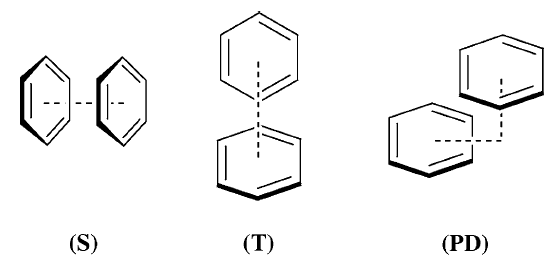
\includegraphics[scale=0.8]{image/Prot} \label{figprot}
		\caption[Structures du dimère de Benzène]{Structures des dimères de Benzène : (S) Sandwich, (T) En forme de T et (PD) Parallèle Déplacé}
	\end{figure}
	
	L’analyse de ces travaux montre que le débat pour estimer quelle est la conformation la plus stable est loin d’être clos. La majorité des travaux rapportent que ce sont les formes T et PD qui sont les plus stables. Pourtant, intuitivement il ne serait pas illogique de penser que la configuration en sandwich, qui correspond à la superposition maximal des deux monomères, puisse apparaitre comme suffisament stable du fait de la maximisation des interactions dispersives. La configuration parallèle déplacée est, quand à elle, souvent observée dans les expériences réalisées à l’état cristallin de composés purement aromatiques \cite{hunter1991pi,fyfe1997synthetic,rebek1996assembly} ou dans les études cherchant à caractériser les interactions des chaînes latérales aromatiques de protéines \cite{hunter1991pi,burley1985aromatic}.Klemperer et al \cite{janda1975benzene} ont, quand à eux, rapportés que la configuration en T était prédominante à l’état gazeux. D’autres travaux issus de l’analyse des spectres rotationnel d'Arunan et Gutowsky \cite{arunan1993rotational}, en accord avec les études Raman de Henson et al \cite{henson1992raman} rapportent que les structures favorables du dimère du benzène s’approchent de la conformation T sans pour autant la confirmer.\\ 
	
	
	Il existe dans la littérature une très grande variété d’approches concernant l’étude des dimères du benzène. Nous faisons le choix de ne reporter, dans le tableau ci-dessous, que les modélisations conduisant aux résultats, à priori du fait des méthodes employées, les plus précis et qui font référence. Les travaux de Park et Lee \cite{park2006accurate}, de Tsuzuki et al \cite{tsuzuki2002origin} et de Sinnokrot et al \cite{hobza1996potential} ont tous été obtenus a partir de calculs CCSD(T) avec extrapolation CBS de base (en anglais Complete Basis Set extrapolation). Cette méthodologie est une technique de calcul empirique basée sur un minimum de trois calculs séparés avec des bases de plus en plus complètes telles que les bases de type cc-pVXZ (X=T, Q, 5 …). Cette technique est une estimation approchée d’un résultat obtenu en utilisant une base infini. Elle permet d’atteindre la limite de précision de la méthode de calcul la plus performante. Nous avons reportés dans le tableau les résultats que nous avons obtenus sur la forme PD qui est celle qui à priori nous intéresse en priorité puisque c’est celle qui a été caractérisée expérimentalement à l’état solide (comme le seront les structures que nous aurons à modéliser dans notre travail issus des données IR obtenues en photo acoustiques). On peut remarquer, en accord avec toutes les données actuellement disponibles sur les approches SAPT, que notre valeur d’énergie d’interaction calculée en SAPT(PBE0)/aug-cc-pVTZ est totalement conforme à la valeur attendue. Sans surprise, l’approche SAPT permet donc de reproduire avec une excellente vélocité les énergies d’interaction de systèmes en interaction pi-pi et d’atteindre la précision nécessaire pour reproduire des données aussi faibles que 1 à 2 kcal/mol.
	
	\begin{table}[H]
		\caption{Energie d'interaction du dimère de Benzène avec CCSD(T) en kcal/mol et DFT-SAPT (PBE0)}
		\begin{center}
			\begin{tabular}{l c r r r c r r c r r r}
				\toprule
				& & & \multicolumn{2}{p{2cm}}{\centering S}  &	& \multicolumn{2}{p{2cm}}{\centering
					T}& &\multicolumn{3}{p{3cm}}{\centering PD}\\
				\cline{4-12}
				& & & & R & &  &  R & & & R$_{1}$ & R$_{2}$ \\
				\midrule
				Park et Lee$^{1}$ & & & &  & &-2,67& 5,0 & &-3,03 & 3,5 & 1,8\\
				Tsuzuki et al$^{2}$ & & & -1,48& 3,8 &  &-2,46& 5,0&  & -2,48 & 3,5& 1,8\\
				Sinnokrot et al$^{3}$ & & & -1,81 & 3.8 & &-2,74& 5,0&  & -2,78 & 3,4 & 1,6\\
				Hobza et al$^{4}$ & & &-1,12 & 4.1 &  &-2,17& 5,1& & -2,01 & 3,6 & 1.8\\
				Sherrill et al$^{5}$& &  & -1,65 & 3,9 & & -2,69& 5,0 & & -2,67 & 3,5 & 1,7 \\
				Rocca$^{6}$ & & & -1,06& 3,9& & -2,15& 5,0 & & -1,82 & 3,4 & 1,8\\ 
				DFT-SAPT (PBE0) & & & -1,47 & 3.9 &  &-2,44 &5,0& & -2,35& 3,5 &1,7\\
				\bottomrule
			\end{tabular}
		\end{center}
		\centering
		\footnotemark[1]{ref \cite{park2006accurate}},
		\footnotemark[2]{ref \cite{tsuzuki2002origin}},
		\footnotemark[3]{ref \cite{sinnokrot2002estimates}},
		\footnotemark[4]{ref \cite{hobza1996potential}}
		\footnotemark[5]{ref \cite{sherrill2009assessment}}
		\footnotemark[6]{ref \cite{rocca2014random}}
		
		[1] CCSD(T)/CBS
		[2] CCSD(T)/CBS 
		[3] CCSD(T)/CBS
		[4] CCSD(T)/aug-cc-pVDZ
		[5] CCSD(T)/CBS 
		[6] RPA
		[7] SAPT(PBE0)/aug-cc-pVTZ (notre travail)
		
		\label{benzene}
	\end{table}
	
	
	
	
	
	
	
	
	
	
	
	\newpage
	%%%%%%%%%%%%%%%%%%%%%%%%%%%%%%%%%%%%%%%%%%%%%%
	%%%%%%%%%%%%%%%%%%%%%%%%%%%%%%%%%%%%%%%%%%%%%%
	%%%%%%%%%%%%%%%%%%%%%%%%%%%%%%%%%%%%%%%%%%%%%%
	%%%%%%%%%%%%%%%%%%%%%%%%%%%%%%%%%%%%%%%%%%%%%%
	\section[DFT]{De la nécessité de la DFT}
	%%%%%%%%%%%%%%%%%%%%%%%%%%%%%%%%%%%%%%%%%%%%%%
	%%%%%%%%%%%%%%%%%%%%%%%%%%%%%%%%%%%%%%%%%%%%%%
	%%%%%%%%%%%%%%%%%%%%%%%%%%%%%%%%%%%%%%%%%%%%%%
	%%%%%%%%%%%%%%%%%%%%%%%%%%%%%%%%%%%%%%%%%%%%%%
	
	Dans ce chapitre, nous rappellerons dans un premier temps les fondements de la théorie de la fonctionnelle de la densité, notée DFT, par le biais de l'évolution des différents modèles qui ont été proposés. Nous verrons ensuite comment les théorèmes de \textsc{Hohenberg} et \textsc{Kohn} prouvent que la seule connaissance de la densité électronique permet de résoudre l'équation de Schr\"{o}dinger dans le cadre de la DFT. La fonctionnelle universelle $F_{HK}[\rho]$, qui permettrait une résolution exacte du problème, restant inconnue, nous aborderons dans une troisième sous partie l'approche KS qui contourne ce problème et légitime certaines approximations. Ces dernières donnant naissance à différents types de fonctionnelle, elles seront succintement présentées dans l’avant dernière sous-partie de ce chapitre. Finalement, nous présenterons la notion de fonctionnelle hybride puis présenterons le principe des approches qui ajoutent \textit{ad hoc} des fonctions semi-empiriques rendant compte des effets de dispersion à un calcul KS usuel.
	
	%%%%%%%%%%%%%%%%%%%%%%%%%%%%%%%%%%%%%%%%%%%%%%
	%%%%%%%%%%%%%%%%%%%%%%%%%%%%%%%%%%%%%%%%%%%%%%
	%%%%%%%%%%%%%%%%%%%%%%%%%%%%%%%%%%%%%%%%%%%%%%
	\subsection{Les fondements de la DFT}
	%%%%%%%%%%%%%%%%%%%%%%%%%%%%%%%%%%%%%%%%%%%%%%
	%%%%%%%%%%%%%%%%%%%%%%%%%%%%%%%%%%%%%%%%%%%%%%
	%%%%%%%%%%%%%%%%%%%%%%%%%%%%%%%%%%%%%%%%%%%%%%
	
	Contrairement aux méthodes Hartree-Fock, noté HF, et \textit{a fortiori} post-HF qui décrivent le système électronique par une fonction d'onde $\Psi_{(\vec{r})}$, la théorie de la fonctionnelle de la densité le décrit par la densité électronique, notée $\rho_{(\vec{r})}$, qui est liée à la fonction d'onde $\Psi_{(\vec{r})}$ par la relation suivante~:
	
	\begin{align}
	\rho_{(\vec{r})} &= \int \Psi_{(\vec{r})}^{*} \Psi_{(\vec{r})} \\
	&= \int |\Psi_{(\vec{r})}^{2}| \notag
	\end{align}
	
	\begin{flushleft}
		\begin{tabular}{@{}lrp{10cm}}
			avec & $\vec{r}$ : & ensemble des coordonnées électroniques. 
		\end{tabular}
	\end{flushleft}
	
	
	L'énergie de l'état fondamental est ainsi une fonctionnelle de la densité électronique, c'est-à-dire que $E_{0} = E_{(\rho)}$.
	
	%%%%%%%%%%%%%%%%%%%%%%%%%%%%%%%%%%%%%%%%%%%%%%
	%%%%%%%%%%%%%%%%%%%%%%%%%%%%%%%%%%%%%%%%%%%%%%
	\subsubsection{Modèle de \textsc{Thomas-Fermi}}
	%%%%%%%%%%%%%%%%%%%%%%%%%%%%%%%%%%%%%%%%%%%%%%
	%%%%%%%%%%%%%%%%%%%%%%%%%%%%%%%%%%%%%%%%%%%%%%
	
	Le terme d'énergie cinétique a été exprimé comme une fonctionnelle de la densité pour la première fois en 1927 par \textsc{Thomas} et \textsc{Fermi}~:
	
	\begin{equation}
	\hat{T}_{TF}[\rho] = \frac{3}{10} (3\pi)^{2/3} \int \rho_{(\vec{r})}^{5/3} .d\vec{r}
	\label{ener_cin_thom_ferm}
	\end{equation}
	
	Celle fonctionnelle est alors combinée aux expressions classiques des interactions électrons-noyaux et électrons-électrons, exprimées elles aussi en fonction de la densité électronique :
	
	\begin{equation}
	E_{TH}[\rho] = T_{TH}[\rho] + V_{Ne}[\rho] + V_{ee}[\rho]
	\end{equation}
	
	%%%%%%%%%%%%%%%%%%%%%%%%%%%%%%%%%%%%%%%%%%%%%%
	%%%%%%%%%%%%%%%%%%%%%%%%%%%%%%%%%%%%%%%%%%%%%%
	\subsubsection{Modèle de \textsc{Thomas-Fermi-Dirac}}
	%%%%%%%%%%%%%%%%%%%%%%%%%%%%%%%%%%%%%%%%%%%%%%
	%%%%%%%%%%%%%%%%%%%%%%%%%%%%%%%%%%%%%%%%%%%%%%
	
	Le terme d'échange, résultant du principe d'exclusion de \textsc{Pauli}, a ensuite été ajouté par Dirac en 1930 afin d'affiner le modèle :
	
	\begin{align}
	K[\rho] = E_{x}[\rho] &= \int \rho_{\vec{r}} \epsilon_{x}[\rho] .d\vec{r} \\
	&= -\frac{3}{4} \left(\frac{3}{\pi}\right)^{1/3} \int \rho_{(\vec{r})}^{4/3} .d\vec{r} \notag
	\end{align}
	
	\begin{flushleft}
		\begin{tabular}{@{}lrp{10cm}}
			avec & $\epsilon_{X}[\rho]$ : & énergie d'échange par électron. 
		\end{tabular}
	\end{flushleft}
	
	Le modèle de \textsc{Thomas-Fermi-Dirac} est défini par la combinaison de cette expression avec l'équation~\ref{ener_cin_thom_ferm} et le potentiel d'interaction électrons-noyaux $V_{Ne}[\rho]$. Notons que la corrélation électronique n'est toujours pas prise en compte dans ce modèle.
	
	
	%%%%%%%%%%%%%%%%%%%%%%%%%%%%%%%%%%%%%%%%%%%%%%
	%%%%%%%%%%%%%%%%%%%%%%%%%%%%%%%%%%%%%%%%%%%%%%
	\subsection{Modèle de \textsc{Slater}}
	%%%%%%%%%%%%%%%%%%%%%%%%%%%%%%%%%%%%%%%%%%%%%%
	%%%%%%%%%%%%%%%%%%%%%%%%%%%%%%%%%%%%%%%%%%%%%%
	
	Partant d'une approche basée sur la méthode HF, \textsc{Slater} proposa en 1951 de substituer le terme d'énergie d'échange par une fonctionnelle de la densité issue de l'énergie d'échange de Dirac. Ce terme d'échange dans le formalisme HF peut alors être généralisé en introduisant le paramètre $\alpha$ :
	
	\begin{equation}
	E_{x}[\rho] = - \frac{9\alpha}{8} \left(\frac{3}{\pi}\right)^{1/3} \int \rho_{(\vec{r})}^{4/3} .d\vec{r}
	\end{equation}
	
	Des analyses empiriques basées sur différents types de systèmes chimiques ont conduit à une valeur de $3/4$ pour $\alpha$, offrant une meilleure précision que la valeur originelle de l'expression de Dirac ($2/3$).
	
	%%%%%%%%%%%%%%%%%%%%%%%%%%%%%%%%%%%%%%%%%%%%%%
	%%%%%%%%%%%%%%%%%%%%%%%%%%%%%%%%%%%%%%%%%%%%%%
	%%%%%%%%%%%%%%%%%%%%%%%%%%%%%%%%%%%%%%%%%%%%%%
	\subsection{Les théorèmes de \textsc{Hohenberg} et \textsc{Kohn}}
	%%%%%%%%%%%%%%%%%%%%%%%%%%%%%%%%%%%%%%%%%%%%%%
	%%%%%%%%%%%%%%%%%%%%%%%%%%%%%%%%%%%%%%%%%%%%%%
	%%%%%%%%%%%%%%%%%%%%%%%%%%%%%%%%%%%%%%%%%%%%%%
	
	Tous ces modèles, qui constituent les fondements de la DFT, ne démontrent pas formellement que seul la connaisance de la densité est importante pour atteindre la valeur de l'énergie totale d'un système. C'est ainsi que \textsc{Hohenberg} et \textsc{Kohn} eurent l'idée en 1965 de démontrer, par le biais de deux théorèmes, que l'équation de Schr\"{o}dinger pouvait être résolue de façon exacte, dans le cadre de l'approximation de \textsc{Born-Oppenheimer} uniquement grâce à la densité électronique.
	
	%%%%%%%%%%%%%%%%%%%%%%%%%%%%%%%%%%%%%%%%%%%%%%
	%%%%%%%%%%%%%%%%%%%%%%%%%%%%%%%%%%%%%%%%%%%%%%
	\subsubsection{Premier théorème : preuve d'existence}
	%%%%%%%%%%%%%%%%%%%%%%%%%%%%%%%%%%%%%%%%%%%%%%
	%%%%%%%%%%%%%%%%%%%%%%%%%%%%%%%%%%%%%%%%%%%%%%
	
	Ce premier théorème énonce que l'ensemble des propriétés du système, notamment l'énérgie, peuvent être calculées à partir de la seule densité électronique de l'état fondamental. Elles peuvent donc être décrites comme une fonctionnelle de la densité électronique, et l'énergie totale s'écrit alors :
	
	\begin{equation}
	E[\rho] = F_{HK}[\rho] + \int \rho_{(\vec{r})} \nu_{ext} .d\vec{r}
	\label{Hohen_Kohn}
	\end{equation}
	\noindent où :
	\begin{align}
	F_{HK}[\rho] &= T_{e}[\rho] + V_{ee}[\rho] \\
	\nu_{ext} &= V_{Ne}[\rho] \notag
	\end{align}
	
	Notons que la fonctionnelle universelle $F_{HK}[\rho]$, qui regroupe les termes d'énergie cinétique des électrons et celui d'énergie potentielle d'interaction électron-électron, n'est pas liée au potentiel externe $\nu_{ext}$. L'énergie de l'état fondamental est \textit{a priori} accessible de manière exacte car cette fonctionnelle ne repose sur aucune approximation.
	
	%%%%%%%%%%%%%%%%%%%%%%%%%%%%%%%%%%%%%%%%%%%%%%
	%%%%%%%%%%%%%%%%%%%%%%%%%%%%%%%%%%%%%%%%%%%%%%
	\subsection{Second théorème : théorème variationnel}
	%%%%%%%%%%%%%%%%%%%%%%%%%%%%%%%%%%%%%%%%%%%%%%
	%%%%%%%%%%%%%%%%%%%%%%%%%%%%%%%%%%%%%%%%%%%%%%
	
	Basé sur l'équation~\ref{Hohen_Kohn}, \textsc{Hohenberg} et \textsc{Kohn} ont ensuite construit un principe variationnel pour déterminer la densité électronique de l'état fondamental :
	
	\begin{equation}
	E[\rho] \geq E[\rho_{0}]
	\end{equation}
	
	\begin{flushleft}
		\begin{tabular}{@{}lrp{10cm}}
			avec & $\rho_{0}$ : & densité électronique de l'état fondamental, \\
			& $\rho$ : & densité électronique quelconque.
		\end{tabular}
	\end{flushleft}
	
	Dans cette équation, à une densité d'essai $\rho$ correspond une seule énergie potentielle $\int \rho_{(\vec{r})} \nu_{ext} .d\vec{r}$ et une seule fonction d'onde $\Psi_{\rho}$. La méthode de double minimisation, \textit{i.e.} sous contrainte de \textsc{Levy}, permet de différencier la fonction d'onde $\Psi_{\rho_{0}}$, correspondant à l'état fondamental, parmi le jeu infini des fonctions d'ondes $\Psi_{\rho}$ donnant la même densité. Ainsi, nous pouvons déterminer, parmi toutes les densités, celle qui minimisera l'énergie par la relation suivante :
	
	\begin{equation}
	E[\rho_{0}] = \min\limits_{\rho}\, (\min\limits_{\Psi\rightarrow\rho}\, (F[\rho] + \int \rho_{\vec{r}} \nu_{\vec{r}}\, .d\vec{r}\, ))
	\end{equation}
	
	Si les théorèmes de \textsc{Hohenberg} et \textsc{Kohn} démontrent une correspondance unique entre une densité $\rho_{\vec{r}}$ et la fonction d'onde $\Psi$ du système, la fonctionnelle universelle $F_{HK}[\rho]$ reste cependant inconnue.
	
	%%%%%%%%%%%%%%%%%%%%%%%%%%%%%%%%%%%%%%%%%%%%%%
	%%%%%%%%%%%%%%%%%%%%%%%%%%%%%%%%%%%%%%%%%%%%%%
	%%%%%%%%%%%%%%%%%%%%%%%%%%%%%%%%%%%%%%%%%%%%%%
	\subsection{Approche Kohn-Sham}\label{Kohn-Sham}
	%%%%%%%%%%%%%%%%%%%%%%%%%%%%%%%%%%%%%%%%%%%%%%
	%%%%%%%%%%%%%%%%%%%%%%%%%%%%%%%%%%%%%%%%%%%%%%
	%%%%%%%%%%%%%%%%%%%%%%%%%%%%%%%%%%%%%%%%%%%%%%
	
	Afin de contourner ce problème, Kohn et Sham substituèrent au Hamiltonien réel, décrivant un système de $n$ particules en interaction, un Hamiltonien de référence décrivant un système de $n$ particules sans interaction mais ayant la même densité que le système réel. Le problème est ainsi réduit à la résolution de $n$ équations monoélectronique couplées, analogues aux équations de HF. L'opérateur monoélectronique de Kohn-Sham $\hat{K}_{KS}$ s'exprime ainsi :
	
	\begin{equation}
	\hat{H}_{KS} = -\frac{1}{2} \nabla^{2} + \nu_{H}[\rho] + \nu_{xc}[\rho] + \nu_{ext}[\rho]
	\end{equation}
	
	\noindent où :
	\begin{align}
	\nu_{H}[\rho] &= \int \frac{\rho_{(\vec{r})} - \rho_{(\vec{r}')}}{|\vec{r} - \vec{r}'|} .d\vec{r}' \\
	\nu_{xc}[\rho] &= \frac{\partial E_{xc}[\rho_{(\vec{r})}]}{\partial\rho_{(\vec{r})}}
	\end{align}
	
	\noindent $\nu_{H}[\rho]$ et $\nu_{xc}[\rho]$ étant respectivement le potentiel de Hartree et le potentiel d'échange et de corrélation, dans lequel $E_{xc}[\rho_{(\vec{r})}]$ est l'énergie d'échange et de corrélation.
	
	En définissant un potentiel fictif $\nu_{eff(\vec{r})}$ pouvant être appliqué à des systèmes sans interaction de densité $\rho$ :
	
	\begin{equation}
	\nu_{eff(\vec{r})} = \nu_{H}[\rho] + \nu_{xc}[\rho] + \nu_{ext}[\rho]
	\end{equation}
	
	\noindent nous introduisons alors un jeu d'orbitales $\psi_{(\vec{r})}$, appelées orbitales de \textsc{Kohn-Sham}, et nous obtenons un jeu d'équations aux valeurs propres :
	
	\begin{equation}
	\hat{H}_{KS} \psi_{i(\vec{r})} = \epsilon_{i} \psi_{i(\vec{r})}
	\end{equation}
	
	Comme dans le cas de la méthode HF, l'énergie du système peut être minimisée en résolvant ce jeu d'équations de façon auto-cohérente grâce à l'utilisation des orbitales de \textsc{Kohn-Sham}. L'énergie du système est alors donnée par :
	
	\begin{equation}
	E_{KS}^{tot}[\rho] = T_{s}[\rho] + J[\rho] + E_{xc}[\rho] + \int V_{ext(\vec{r})}\rho_{(\vec{r})} .d\vec{r}
	\end{equation}
	
	\begin{flushleft}
		\begin{tabular}{@{}lrp{10cm}}
			avec & $T_{s}[\rho]$ : & énergie cinétique des électrons sans interaction, \\
			& $J[\rho]$ : & énergie d'interaction coulombienne entre les électrons, \\
			& $E_{xc}[\rho]$ : & énergie d'échange et de corrélation, \\
			& $\int V_{ext(\vec{r})}\rho_{(\vec{r})} .d\vec{r}$ : & énergie d'interaction avec le potentiel externe. 
		\end{tabular}
	\end{flushleft}
	
	D'après les théorèmes de Hohenberg et Kohn, $E_{KS}^{tot}[\rho]$ doit être égale à l'énergie totale du système réel $E_{reel}^{tot}[\rho]$, qui peut être décrite comme suit :
	
	\begin{equation}
	E_{reel}^{tot}[\rho] = T[\rho] + V_{ee}[\rho] + \int V_{ext(\vec{r})}\rho_{(\vec{r})} .d\vec{r}
	\end{equation}
	
	Le terme d'échange corrélation peut ainsi être explicité comme étant la somme de la correction à l'énergie cinétique due à l'interaction entre électrons ($T[\rho] - T_{s}[\rho]$) et les corrections non classiques à la répulsion électron-électron ($V_{ee}[\rho] - J[\rho]$) :
	
	\begin{equation}
	E_{xc}[\rho] = T[\rho] - T_{s}[\rho] + V_{ee}[\rho] - J[\rho]
	\end{equation}
	
	La théorie de la fonctionnelle de la densité de Kohn-Sham (KS) a connu un grand succès parmi les méthodes de calcul appliquées aux grands systèmes dû à son ratio coût calculatoire/performance très intéressant. C'est pour cet avantage indéniable qu'elle sert de base à de nombreuses évolutions de la DFT.
	
	%%%%%%%%%%%%%%%%%%%%%%%%%%%%%%%%%%%%%%%%%%%%%%
	%%%%%%%%%%%%%%%%%%%%%%%%%%%%%%%%%%%%%%%%%%%%%%
	%%%%%%%%%%%%%%%%%%%%%%%%%%%%%%%%%%%%%%%%%%%%%%
	\subsection{Les différentes classes de fonctionnelle}
	%%%%%%%%%%%%%%%%%%%%%%%%%%%%%%%%%%%%%%%%%%%%%%
	%%%%%%%%%%%%%%%%%%%%%%%%%%%%%%%%%%%%%%%%%%%%%%
	%%%%%%%%%%%%%%%%%%%%%%%%%%%%%%%%%%%%%%%%%%%%%%
	
	Formellement, la DFT est donc une méthode exacte, dans la limite de la connaissance de la fonctionnelle universelle $F_{HK}[\rho]$ ou de sa fonctionnelle exacte d’échange et de corrélation $F_{xc}[\rho]$. Malheureusement, la forme exacte de l’énergie d’échange et de corrélation est inconnue, si bien qu’il est nécessaire de faire des approximations. Dans la pratique, l’énergie d’échange et de corrélation $E_{xc}[\rho]$ est calculée à l’aide de fonctionnelles d’échange et de corrélation, définies comme suit :
	
	\begin{equation}
	\int F_{xc}[\rho_{(\vec{r})}].d\vec{r} = E_{xc}[\rho_{(\vec{r})}]
	\end{equation}
	
	L’énergie d’échange et de corrélation est généralement séparée en deux termes distincts, l’un d’échange $E_{x}[\rho]$ et l’autre de corrélation $E_{c}[\rho]$ :
	
	\begin{equation}
	E_{xc}[\rho_{(\vec{r})}] = E_{x}[\rho_{(\vec{r})}] + E_{c}[\rho_{(\vec{r})}]
	\end{equation}
	
	Plusieurs fonctionnelles ont donc été développées pour traiter chacune de ces contributions, de façon simultanée ou indépendante. Nous allons ici donner un bref aperçu -- non exhaustif -- des différentes familles de fonctionnelles, en suivant le critère de classification donné par Perdew et couramment dit \og échelle de Jacob de Perdew \fg{}. Il a proposé de classer les fonctionnelles en fonction du degré d’information non local contenu dans leur forme analytique. Au premier échelon se trouvent les fonctionnelles qui dépendent uniquement de la densité électronique, dites fonctionnelles LDA (\og Local Density Approximation \fg{}). Viennent ensuite les fonctionnelles corrigées par gradient GGA (\og Generalized Gradient Approximation \fg{}) dans lesquelles la non-localité est introduite grâce à leur dépendance par rapport au gradient de la densité. A ce même niveau se trouvent également les fonctionnelles de type méta-GGA, dépendant aussi de l’énergie cinétique (calculée à partir des orbitales moléculaires remplies). Il faut noter que, d’un point de vue mathématique, toutes ces familles de fonctionnelles sont strictement locales. Pour parvenir à des fonctionnelles véritablement non locales il faut encore monter d’un cran dans l’échelle de Perdew, jusqu’aux fonctionnelles dites hybrides, où la présence d’un pourcentage (variable) d’échange HF calculé en utilisant les orbitales KS, permet d’introduire un véritable terme non local. Plus récemment une autre famille de fonctionnelles hybrides a été développée (dite à longue portée ou encore à séparation de portée) dans laquelle le pourcentage d’échange calculé de façon HF n’est pas constant mais dépend de la distance inter-électronique. Enfin, des fonctionnelles non locales montrant une dépendance explicite des orbitales KS occupées et vacantes représentent le dernier niveau dans l’échelle de Perdew.
	
	%%%%%%%%%%%%%%%%%%%%%%%%%%%%%%%%%%%%%%%%%%%%%%
	%%%%%%%%%%%%%%%%%%%%%%%%%%%%%%%%%%%%%%%%%%%%%%
	\subsubsection{Local Density approximation (LDA)}\label{lda}
	%%%%%%%%%%%%%%%%%%%%%%%%%%%%%%%%%%%%%%%%%%%%%%
	%%%%%%%%%%%%%%%%%%%%%%%%%%%%%%%%%%%%%%%%%%%%%%
	
	L’approximation locale de la densité est l’approximation la plus grossière, dans laquelle l’énergie d’échange et de corrélation $E_{xc}$ n’est fonction que de la seule densité électronique :
	
	\begin{equation}
	E_{xc}^{LDA}[\rho_{(\vec{r})}] = \int \rho_{(\vec{r})} \epsilon_{xc}[\rho_{(\vec{r})}].d\vec{r}
	\end{equation}
	
	\noindent où la valeur de $\epsilon_{xc}$ à une position $\vec{r}$ est calculée exclusivement à partir de la valeur de la densité électronique $\rho$ à cette position. En pratique, $\epsilon_{xc}$ décrit l’énergie d’échange et de corrélation par particule pour un gaz uniforme d’électrons de densité $\rho$. Le potentiel d’échange et de corrélation correspondant est alors :
	
	\begin{equation}
	\nu_{xc(\vec{r})}^{LDA} = \epsilon_{xc}[\rho_{(\vec{r})}] + \rho_{(\vec{r})} \frac{\partial \epsilon_{xc}[\rho_{(\vec{r})}]}{\partial \rho}
	\end{equation}
	
	Malgré le fait que les résultats obtenus soient généralement en bon accord avec les résultats expérimentaux, notamment au niveau de la géométrie et de la structure électronique, cette approximation reste une approximation locale, c'est-à-dire dans laquelle on ne tient pas compte de l’inhomogénéité de la densité électronique.
	
	%%%%%%%%%%%%%%%%%%%%%%%%%%%%%%%%%%%%%%%%%%%%%%
	%%%%%%%%%%%%%%%%%%%%%%%%%%%%%%%%%%%%%%%%%%%%%%
	\subsubsection{Generalized Gradient Approximation (GGA)}
	%%%%%%%%%%%%%%%%%%%%%%%%%%%%%%%%%%%%%%%%%%%%%%
	%%%%%%%%%%%%%%%%%%%%%%%%%%%%%%%%%%%%%%%%%%%%%%
	
	L’idée directrice de l’approximation du gradient généralisé est donc de mieux tenir compte de l’inhomogénéité de la densité du système, en introduisant une dépendance de la densité $\rho$ à son gradient $\nabla \rho$. L’expression générale des fonctionnelles de type GGA est la
	suivante :
	
	\begin{equation}
	E_{xc}^{GGA}[\rho_{(\vec{r})}] = A_{x} \int \rho_{(\vec{r})}^{4/3} E^{GGA}(s) .d\vec{r}^{3}
	\end{equation}
	
	\noindent où $s$, gradient de la densité réduite, est tel que :
	
	\begin{equation}
	s = \frac{|\nabla \rho_{(\vec{r})}|}{2 k_{F} \rho_{(\vec{r})}}
	\end{equation}
	
	\noindent avec $k_{F} = (3 \pi^{2} \rho_{(\vec{r})})^{1/3}$. Ainsi, on fait apparaître avec $s$ un terme quasi-local, dépendant non seulement de la densité électronique mais également de son gradient au voisinage de $\vec{r}$.
	
	Un exemple de fonctionnelle GGA est celle de \textsc{Perdew}, \textsc{Burke} et \textsc{Ernzherhof}, notée PBE~\cite{perdew1996generalized}.
	
	%%%%%%%%%%%%%%%%%%%%%%%%%%%%%%%%%%%%%%%%%%%%%%
	%%%%%%%%%%%%%%%%%%%%%%%%%%%%%%%%%%%%%%%%%%%%%%
	\subsubsection{Fonctionnelles hybrides}
	%%%%%%%%%%%%%%%%%%%%%%%%%%%%%%%%%%%%%%%%%%%%%%
	%%%%%%%%%%%%%%%%%%%%%%%%%%%%%%%%%%%%%%%%%%%%%%
	
	La dernière grande famille de fonctionnelles est celle des fonctionnelles hybrides. L’idée consiste à introduire une fraction d’échange calculée de façon exacte (telle qu’utilisée dans la méthode HF) dans une fonctionnelle d’échange de type GGA. L’expression de $E_{xc}$ devient alors :
	
	\begin{equation}
	E_{xc}^{hybride}[\rho_{(\vec{r})}] = (1- \alpha) E_{xc}^{GGA}[\rho_{(\vec{r})}] + \alpha E_{xc}^{HF}[\rho_{(\vec{r})}]
	\end{equation}
	
	\noindent où le coefficient de la combinaison $\alpha$ donne le rapport HF/DFT.
	PBE0~\cite{adamo1999toward} Celle-ci présente 25\% d’échange HF~\cite{adamo1997toward} dans une fonctionnelle GGA de type PBE~\cite{perdew1996generalized} :
	
	\begin{equation}
	E_{xc}^{PBE0} = E_{xc}^{PBE} + \frac{1}{4} (E_{x}^{HF} - E_{x}^{PBE})
	\end{equation}
	
	Elle a l’avantage d’être non paramétrée (car le pourcentage d’HF inclus n’est pas empirique mais basé sur des arguments de théorie perturbationnelle), et de fournir des résultats très précis, que ce soit au niveau du calcul des structures moléculaires, des structures électroniques ou encore des propriétés spectroscopiques \cite{adamo1999toward}.
	
	Nous mentionnerons également la fonctionnelle hybride la plus utilisée pour traiter des systèmes moléculaires, à savoir la fonctionnelle B3LYP \cite{becke1993density}. Comme son nom l’indique, elle inclus trois paramètres et est basée sur les fonctionnelles GGA d’échange et de corrélation de \textsc{Becke} (B) \cite{becke1988density} et \textsc{Lee}, \textsc{Yang} et \textsc{Parr} (LYP) \cite{chengteh1988development}, suivant l’expression :
	
	\begin{equation}
	E_{xc}^{B3LYP} = (1-a) E_{x}^{LSDA} + a E_{x}^{HF} + b \Delta E_{x}^{B} + (1-c) E_{c}^{LSDA} + c E_{c}^{LYP}
	\label{B3LYP}
	\end{equation}
	
	\noindent avec $a$, $b$ et $c$ fixés respectivement à 0,20 , 0,72 et 0,81.
	
	
	%%%%%%%%%%%%%%%%%%%%%%%%%%%%%%%%%%%%%%%%%%%%%%
	%%%%%%%%%%%%%%%%%%%%%%%%%%%%%%%%%%%%%%%%%%%%%%
	\subsubsection{Nécessité d'une fonctionnelle « longue portée »}
	%%%%%%%%%%%%%%%%%%%%%%%%%%%%%%%%%%%%%%%%%%%%%%
	%%%%%%%%%%%%%%%%%%%%%%%%%%%%%%%%%%%%%%%%%%%%%%
	
	Même si la théorie de la fonctionnelle de la densité connaît un large succès il lui reste toujours, en particulier, l'obstacle des systèmes chimiques où les forces de Van der Waals sont prédominantes. En effet, les effets de corrélation électronique des forces de dispersion étant purement non-locaux, l'approximation locale ou non-locale qui fait le fondement de la DFT restera problématique. Se pose alors la question de savoir comment modéliser ces types d'interaction de façon idiomatique. Nous allons voir que l'élaboration d'une fonctionnelle hybride à longue portée est capable de répondre, au premier degrés de l’échelle de précision, à cette problématique.
	
	%%%%%%%%%%%%%%%%%%%%%%%%%%%%%%%%%%%%%%%%%%%%%%
	%%%%%%%%%%%%%%%%%%%%%%%%%%%%%%%%%%%%%%%%%%%%%%
	%%%%%%%%%%%%%%%%%%%%%%%%%%%%%%%%%%%%%%%%%%%%%%
	\subsection[LC-DFT-D hybride : $\omega$BXD]{Construction d'une LC-DFT-D hybride : cas de la $\omega$BXD}
	%%%%%%%%%%%%%%%%%%%%%%%%%%%%%%%%%%%%%%%%%%%%%%
	%%%%%%%%%%%%%%%%%%%%%%%%%%%%%%%%%%%%%%%%%%%%%%
	%%%%%%%%%%%%%%%%%%%%%%%%%%%%%%%%%%%%%%%%%%%%%%
	Les DFT hybrides avec correction à longue portée basées sur la théorie \textsc{Kohn-Sham} ont naturellement rencontré un grand engouement puisque la précision apportée n'accroît pas le coût calculatoire par rapport aux DFT hybrides.
	
	%%%%%%%%%%%%%%%%%%%%%%%%%%%%%%%%%%%%%%%%%%%%%%
	%%%%%%%%%%%%%%%%%%%%%%%%%%%%%%%%%%%%%%%%%%%%%%
	\subsubsection{B88}
	%%%%%%%%%%%%%%%%%%%%%%%%%%%%%%%%%%%%%%%%%%%%%%
	%%%%%%%%%%%%%%%%%%%%%%%%%%%%%%%%%%%%%%%%%%%%%%
	
	Comme nous l'avons vu dans le cadre des approximations de la fonctionnelle de la densité, notées DFAs\footnote{\og Density Functional Approximations \fg{} }, la décroissance en exponentielle du potentiel d'échange-corrélation, au lieu d'être en $1/r$, engendre une mauvaise représentation des interactions à longue distance. Cette erreur, nommée erreur d'auto-interaction (SIE, pour \og self-interaction error \fg{}), est liée au fait que ces approximations, basées sur la densité de spin locale (LSDA, pour \og local spin density approximation \fg{}), décrivent mal l'état fondamental qui devrait être, dans le cadre de la DFT pure, strictement sans auto-interaction.     
	C'est pourquoi, afin d'introduire un effet non-local de l'échange-corrélation dans le modèle KS-DFT (partie~\ref{Kohn-Sham}), \textsc{Becke} proposa en 1988 d'incorporer dans sa fonctionnelle d'échange B88~\cite{becke1988density} une petite part d'echange exact \textsc{Hartree-Fock}. 
	
	Dans le cadre général des DFAs, l'énergie d'échange-corrélation s'écrit donc :
	
	\begin{equation}
	E_{xc} = c_{x}E_{x}^{HF} + E_{xc}^{DFA}
	\label{xcB88}
	\end{equation}
	
	\noindent où $c_{x}$ prend généralement des valeurs comprises entre 0,2 et 0,25~\cite{becke1993density} pour traduire au mieux les données thermodynamiques et entre 0,4 et 0,6~\cite{boese2004development} pour traduire au mieux les études cinétiques.
	
	Basée sur ce modèle, la désormais bien connue DFT hybride B3LYP \cite{becke1993density} (équation~\ref{B3LYP}) donne des résultats comparables à ceux obtenus à partir de la théorie perturbative \textsc{M\o ller-Plesset} à l'ordre 2 \cite{moller1934note}, noté MP2, souvent utilisée comme référence, dans le cadre de systèmes fortement liés. Depuis, de nombreuses recherches ont porté sur l'amélioration constante de ce potentiel d'échange-corrélation $E_{xc}[\rho]$.
	
	Je ne saurai continuer ce paragraphe sans attirer l’attention sur le caractère quelque peu ‘erratique’ observé dans la majorité des travaux publiés en DFT, caractère issu du choix de la fonctionnelle d’échange et/ou de corrélation. Si pour un système donné une fonctionnelle d’échange-corrélation est capable de produire des paramètres satisfaisants autour de la position d’équilibre, il n’est pratiquement jamais garanti qu’elle soit en mesure de donner la même précision pour un autre (type de) système, et qui plus est pour l’étude de dimères (atomiques ou moléculaires). Une attention toute particulière a donc été portée initialement dans notre travail sur le choix de la fonctionnelle d’échange-corrélation puisqu’il s’agissait de pouvoir étudier une très grande variété de systèmes i.e. non seulement des familles de molécules comportant un ou plusieurs hétéroatome(s) mais les homo-dimères correspondant. La fonctionnelle $\omega$b97X a retenue notre attention dans ce travail.
	
	
	%%%%%%%%%%%%%%%%%%%%%%%%%%%%%%%%%%%%%%%%%%%%%%
	%%%%%%%%%%%%%%%%%%%%%%%%%%%%%%%%%%%%%%%%%%%%%%
	\subsubsection{B97}
	%%%%%%%%%%%%%%%%%%%%%%%%%%%%%%%%%%%%%%%%%%%%%%
	%%%%%%%%%%%%%%%%%%%%%%%%%%%%%%%%%%%%%%%%%%%%%%
	
	Une avancée significative a de nouveau été faite par \textsc{Becke} en 1997 dans le domaine des KS-DFT. Par une méthode similaire à la combinaison linéaire d'orbitales atomiques, notée LCAO\footnote{\og Linear Combination of Atomic Orbitals \fg{}.}, Becke a proposé un modèle mathématique basé sur l'approximation de densité de spin local (LSDA), sa première dérivée et une petite fraction d'échange HF pour décrire le potentiel d'échange-corrélation $E_{xc}[\rho]$. Une optimisation systématique des coefficients linéaires à partir d'un jeu classique de données expérimentales a conduit à l'apparition de la méthode B97~\cite{becke1997density}. La base de données contient notamment des valeurs relatives à l'interaction entre systèmes conjugués.
	
	Cette méthodologie a été reprise par F. A. \textsc{Hamprecht} et al, P. J. \textsc{Wilson} et al et T. W. \textsc{Keal} et al pour respectivement conduire à la B97-1 \cite{hamprecht1998development} (1998), la B97-2 \cite{wilson2001hybrid} (2001) et la B97-3 \cite{keal2005semiempirical} (2005). Il s'agissait alors de réoptimisations des coefficients linéaires par rapport à d'autres bases de données expérimentales plus complètes.
	
	Mais cette reparamétrisation empirique du terme d'échange-corrélation ne résout pas le problème de sa non-décroissance en $1/r$. La prise en compte totale du terme d'échange HF $E_{x}^{HF}$ ($c_{x}$=1 dans l'équation~\ref{xcB88}) pourait résoudre ce problème mais cela serait incompatible avec le terme de corrélation DFA $E_{c}^{DFA}$. En effet, il existerait alors une mauvaise compensation des erreurs respectives.
	
	%%%%%%%%%%%%%%%%%%%%%%%%%%%%%%%%%%%%%%%%%%%%%%
	%%%%%%%%%%%%%%%%%%%%%%%%%%%%%%%%%%%%%%%%%%%%%%
	\subsubsection{$\omega$B97}
	%%%%%%%%%%%%%%%%%%%%%%%%%%%%%%%%%%%%%%%%%%%%%%
	%%%%%%%%%%%%%%%%%%%%%%%%%%%%%%%%%%%%%%%%%%%%%%
	
	L'idée de séparer le traitement des interactions courtes (SR, pour \og short range \fg{}) et longues portées (LR, pour \og long range \fg{}) s'est alors présentée comme le choix le plus évident, aussi bien au niveau de la compréhension des phénomènes que mathématiquement parlant. Nous pouvons ainsi traiter séparément à l'aide d'une fonction erreur $(erf)$ les interactions à courtes distances par une fonctionnelle de la densité et celles longue distance par une fonction d'onde. Ce principe conduit naturellement à l'élaboration d'une fonctionnelle hybride à séparation de portée. L'introduction de la fonction erreur, avec un paramètre libre, permet de contrôler le rayon d'action des interactions de courte-portée.
	
	Une des premières propositions faite a été faite par Iikura et al \cite{iikura2001long}. Elle consiste à traiter la partie d'échange LR par la théorie HF alors que la partie SR est approximée par une DFA; le terme de corrélation est quant à lui le même que celui de \textsc{Coulomb}, quelle que soit la distance :
	
	\begin{equation}
	E_{xc}^{LC-DFA} = E_{x}^{LR-HF} + E_{x}^{SR-DFA} + E_{c}^{DFA}
	\end{equation}
	
	Ce schéma de séparation de portée a l'avantage de conduire à des temps de calcul très proches des DFT hybrides, mais il reste à développer une fonctionnelle d'échange SR précise et une fonctionnelle de corrélation qui soit entièrement compatible entre elles.
	
	Le type d'opérateur de coupure le plus utilisé dans le cadre des LC-DFT hybrides est la fonction d'erreur standard $(erf)$ :
	
	\begin{equation}
	\frac{1}{r} = \frac{erf(\omega r_{12})}{r_{12}} + \frac{erfc(\omega r_{12})}{r_{12}}
	\label{erf}
	\end{equation}
	
	\begin{flushleft}
		\begin{tabular}{@{}lrp{10cm}}
			avec & $\frac{erf(\omega r_{12})}{r_{12}}$ : & interaction de courte portée, \\
			& $\frac{erfc(\omega r_{12})}{r_{12}}$ : & interaction complémentaire, \\
			& $r_{12}$ : & distance entre les particules 1 et 2, \\
			& $\omega$ : & paramètre contrôlant la séparation.
		\end{tabular}
	\end{flushleft}
	
	Notons que l'introduction du paramètre $\omega$, qui s'exprime comme l'inverse d'une distance, permet de donner un sens physique à cette valeur, en cela qu'il est étroitement lié à une longueur caractéristique de la séparation.
	Naturellement, il existe différents types de fonctions erreur $(erf)$ afin de faciliter son intégration mathématique dans les codes de calculs. Dans le cas de la $\omega$B97 \cite{chai2008long} et, par conséquent, des fonctionnelles $\omega$B97X et $\omega$B97X-D, c'est la fonction $erf/erfc$ qui a été choisie par Jeng-Da Chai et Martin Head-Gordon dans leurs travaux. \\
	
	Le choix des auteurs s'est porté sur un terme d'échange exact HF longue portée $E_{x}^{LR-HF}$, calculé à partir des spin-orbitales occupées $\phi_{i \sigma}(r)$, et une forme analytique du terme d'échange $E_{x}^{SR-DFA}$ obtenue par l'intégration du carré de la matrice densité LSDA :
	
	\begin{align}
	E_{x}^{LR-HF} &= -\frac{1}{2} \sum_{\sigma} \sum_{ij}^{occ.} \iint \phi_{i \sigma}^{*}(r_{1}) \phi_{j \sigma}^{*}(r_{1}) \frac{erf(\omega r_{12})}{r_{12}} \phi_{i \sigma}(r_{2}) \phi_{j \sigma}(r_{2}).dr_{1}.dr_{2}, \\
	E_{x}^{SR-LSDA} &= \sum_{\sigma} \int \underbrace{-\frac{3}{2}\left(\frac{3}{4\pi}\right)^{1/3}\rho_{\sigma}^{4/3} (r) F(a_{\sigma})}_{e_{x \sigma}^{SR-LSDA} (\rho_{\sigma}) .dr}.
	\end{align}
	
	\noindent où :
	\begin{align}
	k_{F \sigma}&=(6\pi^{2}\rho_{sigma}(r))^{1/3},\nonumber\\
	F(a_{\sigma})&=1-\frac{8}{3}a_{\sigma}\left[\sqrt{\pi}\: erf\left(\frac{1}{2a_{\sigma}}\right)-3a_{\sigma}+4a_{\sigma}^{3}+(2a_{\sigma}-4a_{\sigma}^{3}) \: exp\left(-\frac{1}{4a_{\sigma}^{2}}\right)\right],\nonumber\\
	a_{\sigma}&=\frac{\omega}{2k_{F\sigma}}.\nonumber
	\end{align}
	
	\begin{flushleft}
		\begin{tabular}{@{}lrp{10cm}}
			avec & $k_{F\sigma}$ : & vecteur d'onde local de Fermi,\\
			& $F(a_{\sigma})$ : & fonction d'atténuation,\\
			& $a_{\sigma}$ : & paramètre de contrôle (sans unité) de la fonction d'atténuation $F(a_{\sigma})$.
		\end{tabular}
	\end{flushleft}
	
	En retenant une fonctionnelle de corrélation basée elle aussi sur la LSDA $E_{c}^{LSDA}$, la plus simple des DFT hybrides à correction de longue portée (RSHX-LDA pour l’anglais Range Separated Hybrid eXchange J. G. Ángyan, I. C. Gerber, A Savin et J Toulouse. « van der Waals forces in densityfunctional theory : Perturbational long-range electron-interaction corrections ». Phys. Rev. A 72 (2005), 012510) s'écrit~:
	
	\begin{equation}
	E_{xc}^{RSHXLDA} = E_{x}^{LR-HF} + E_{x}^{SR-LSDA} + E_{c}^{LSDA}
	\end{equation}
	
	La fonctionnelle $\omega$B97\cite{chai2008long} s'écrit alors :
	
	\begin{equation}
	E_{xc}^{\omega B97} = E_{x}^{LR-HF} + E_{x}^{SR-B97} + E_{c}^{B97}
	\end{equation}
	
	Il est à noter que celle-ci ne possède pas d'échange Hartree-Fock à courte portée (SR), comme la plupart des fonctionnelles hybrides à correction de portée.
	
	Malgré plusieurs études visant à optimiser la valeur du paramètre $\omega$, la précision calculatoire reste insuffisante en terme de thermochimie. En effet, nous l'avons déjà vu, une valeur trop grande pour $\omega$ tendrait vers une incompatibilité entre le terme d'échange non-local $E_{x}^{LR-HF}$ et le terme local de corrélation $E_{c}^{LSDA}$. De plus, nous pouvons aisément comprendre, d'après l'équation~\ref{erf}, que plus $\omega$ est petit, plus la contribution du terme d'échange SR $E_{x}^{SR-LSDA}$ sera importante. L'utilisation d'une trop faible valeur  reviendrait alors à traiter le problème dans un cadre très proche de la LDA classique qui, comme nous l'avons vu dans la partie~\ref{lda}, est incapable de traduire correctement le terme d'échange à courte portée.
	
	%%%%%%%%%%%%%%%%%%%%%%%%%%%%%%%%%%%%%%%%%%%%%%
	%%%%%%%%%%%%%%%%%%%%%%%%%%%%%%%%%%%%%%%%%%%%%%
	\subsubsection{$\omega$B97X}
	%%%%%%%%%%%%%%%%%%%%%%%%%%%%%%%%%%%%%%%%%%%%%%
	%%%%%%%%%%%%%%%%%%%%%%%%%%%%%%%%%%%%%%%%%%%%%%
	
	Afin d'y remédier, une partie d'échange SR HF $E_{x}^{SR-HF}$, est ajoutée à $E_{x}^{SR-LSDA}$ dans une proportion d'environ 16\%,  de la même manière que Becke dans la fonctionnelle B88. Ceci à l'avantage de ne pas perturber la partie LR qui est dorénavant correcte. Ainsi, la nouvelle fonctionnelle comporte désormais un paramètre $c_{x}$ contrôlant la proportion d'échange exact HF à courte distance, comme nous pouvons le voir dans son expression :
	
	\begin{equation}
	E_{xc}^{LC-DFA} = E_{x}^{LR-HF} + c_{x}E_{x}^{SR-HF} + E_{x}^{SR-DFA} + E_{c}^{DFA}
	\end{equation}
	
	\noindent où :
	
	\begin{equation}
	E_{x}^{SR-HF} = -\frac{1}{2} \sum_{\sigma} \sum_{ij}^{occ.} \iint \phi_{i \sigma}^{*}(r_{1}) \phi_{j \sigma}^{*}(r_{1}) \frac{erfc(\omega r_{12})}{r_{12}} \phi_{i \sigma}(r_{2}) \phi_{j \sigma}(r_{2}).dr_{1}.dr_{2}, \\
	\end{equation}
	
	C'est ainsi que la fonctionnelle $\omega$B7X\cite{chai2008long} se décompose de la façon suivante~:
	
	\begin{equation}
	E_{xc}^{\omega B97X} = E_{x}^{LR-HF} + c_{x}E_{x}^{SR-HF} + E_{x}^{SR-B97} + E_{c}^{B97}
	\end{equation}
	
	La valeur de $\omega$, comme les valeurs des coefficients de développements linéaires et de développements à l'ordre $m$ des fonctionnelles $\omega$B97 et $\omega$B97X ont été déterminées par la méthode des moindres carrés appliquée à une base de données composées de 412 valeurs précises, expérimentales et théoriques.
	
	Malgré toutes ces optimisations conduisant à une bien meilleure représentation des systèmes en interaction, ces fonctionnelles connaissent encore des lacunes quant à la traduction des interactions de dispersion entre atomes, ie les forces de London. Comme nous allons le voir dans le cas de la fonctionnelle $\omega$B97X-D, ceci peut être corrigé par une prise en compte empirique des effets de dispersion.
	
	%%%%%%%%%%%%%%%%%%%%%%%%%%%%%%%%%%%%%%%%%%%%%%
	%%%%%%%%%%%%%%%%%%%%%%%%%%%%%%%%%%%%%%%%%%%%%%
	\subsubsection{$\omega$B97X-D}
	%%%%%%%%%%%%%%%%%%%%%%%%%%%%%%%%%%%%%%%%%%%%%%
	%%%%%%%%%%%%%%%%%%%%%%%%%%%%%%%%%%%%%%%%%%%%%%
	
	Cette dernière correction pourrait naturellement passer par le calcul de l'énergie de dispersion entre chaque atome, mais cela occasionnerait alors un coût calculatoire prohibitif. C'est pourquoi Jeng-Da \textsc{Chai} et Martin \textsc{Head-Gordon} ont fait le choix d'appliquer cette correction de façon empirique par l'ajout d'un terme $E_{disp}$ à la fonctionnelle KS-DFT, ici la $\omega$B97X. L'expression de l'énergie de la fonctionnelle $\omega$B97X-D \cite{chai2008long} ainsi créée devient alors :
	
	\begin{equation}
	E_{DFT-D}=E_{\omega B97X}+E_{disp}
	\end{equation}
	
	L'énergie de dispersion $E_{disp}$ est définie par rapport à une fonction d'amortissement $f_{damp}$ :
	
	\begin{equation}
	E_{disp}=-\sum_{i-1}^{N_{at}-1} \sum_{j-i+1}^{N_{at}} \frac{C_{6}^{ij}}{R_{ij}^{6}}f_{damp} (R_{ij})
	\end{equation}
	
	\noindent où :
	\begin{equation}
	f_{damp} (R_{ij})=\frac{1}{1+a(\frac{R_{ij}}{R_{r}})^{-12}}
	\end{equation}
	
	En conclusion, les travaux de Jeng-Da Chai et Martin Head-Gordon ont finalement conduit à la fonctionnelle $\omega$B9X-D, de type LC-DFT-D hybride, où la totalité de l'échange exact HF est pris en compte à longue distance, en même temps qu'une petite partie -- environ 22 \% -- de l'échange exact HF est introduite à courte distance pour compléter une fonctionnelle d'échange B97 modifiée ; une correction empirique de la dispersion est finalement appliquée. La partie empirique a été paramétrée par rapport à la même base de données que pour les fonctionnelles $\omega$B97 et $\omega$BX97.
	
	%%%%%%%%%%%%%%%%%%%%%%%%%%%%%%%%%%%%%%%%%%%%%%
	%%%%%%%%%%%%%%%%%%%%%%%%%%%%%%%%%%%%%%%%%%%%%%
	%%%%%%%%%%%%%%%%%%%%%%%%%%%%%%%%%%%%%%%%%%%%%%
	\subsection{DFT+D}
	%%%%%%%%%%%%%%%%%%%%%%%%%%%%%%%%%%%%%%%%%%%%%%
	%%%%%%%%%%%%%%%%%%%%%%%%%%%%%%%%%%%%%%%%%%%%%%
	%%%%%%%%%%%%%%%%%%%%%%%%%%%%%%%%%%%%%%%%%%%%%%
	
	Les fonctionnelles DFT-D i.e. BLYP-D, B3LYP-D, B97-D, PBE-D (Anthony and Grimme 2006), M05-2x et M06-2x (Zhao and Truhlar 2008) sont traditionnellement incluses dans la famille des fonctionnelles dites \it{semiempirical dispersion-corrected functionals}. En effet, dans ces fonctionnelles les effets de corrélation à longue distance sont purement et simplement traités par la correction empirique de dispersion selon trois niveaux d’empirisme notés respectivement DFT-D1, DFT-D2 et DFT-D3. 
	
	%%%%%%%%%%%%%%%%%%%%%%%%%%%%%%%%%%%%%%%%%%%%%%
	%%%%%%%%%%%%%%%%%%%%%%%%%%%%%%%%%%%%%%%%%%%%%%
	\subsubsection{DFT-D2}
	%%%%%%%%%%%%%%%%%%%%%%%%%%%%%%%%%%%%%%%%%%%%%%
	%%%%%%%%%%%%%%%%%%%%%%%%%%%%%%%%%%%%%%%%%%%%%%
	
	S. Grimme \cite{grimme2006semiempirical} propose en 2006 une première amélioration à sa correction empirique initiale de la dispersion \cite{grimme2004accurate}, appelée D2 dans le but de corriger trois défauts principalement constatés i.e. les coefficients C$_{6}$ n’étaient disponibles dans la version originale que pour les atomes les plus légers de la classification périodique, l’utilisation des données tabulées pour les atomes de la troisième période conduisaient à des erreurs systématiques, et enfin les résultats obtenus ne permettaient pas de retrouver quelques principes usuels de la thermochimie.  
	
	Conformément à ce que nous avons reportés au paragraphe précédent, l’expression de l'énergie de la fonctionnelle s’exprime toujours de la forme :
	
	\begin{equation}
	E_{DFT-D2} = E_{KS-DFT} + E_{disp}^{(2)}
	\end{equation}
	
	L'énergie de dispersion $E_{disp}$ est, quand à elle, toujours définie par rapport à une fonction d'amortissement $f_{damp}$ :
	
	\begin{equation}
	E_{disp}^{(2)}=-s_{6} \sum_{i=1}^{N_{at}-1} \sum_{j=i+1}^{N_{at}} \frac{C_{6}^{ij}}{R_{ij}^{6}} f_{d,6} (R_{ij})
	\end{equation}
	
	\noindent où :
	\begin{equation}
	f_{d,6} (R_{ij})= \frac{s_{6}}{1+exp^{(-d(\frac{R_{ij}}{s_{R}R_{Oij}}-1)}}  
	\end{equation}
		
		dans laquelle le paramètre $s_{6}$ est optimisé selon la selon la fonctionnelle d’échange-corrélation utilisée. Les coefficients de vdW d’ordre 6 et les rayons de vdW des espèces en interaction sont quand à eux calculés à partir des données tabulées sur les atomes selon les expressions suivantes :
		
		\begin{equation}
		C_{6ij} =\sqrt{C_{6ii}C_{6jj}}  
		\end{equation}

\begin{equation}
C_{6ii} = 0.05NI_{p}{i} \alpha_{i}
\end{equation}

et 

\begin{equation}
R_{Oij} = R_{Oi} + R_{Oj}
\end{equation}

Les termes $I_{p}{i}$ et $\alpha_{i}$ représentent respectivement le potentiel d’ionisation atomique et la polarisabilité statique de l’élément $i$.

La correction D2 a été principalement testée par Grimme \cite{grimme2006semiempirical} pour l’étude des systèmes de références que sont les gaz diatomiques, le benzène et les petites molécules aromatiques telle que l’anthracène, etc. Plus tard, Park et al \cite{park2011ab} ont étudiés des systèmes graphitiques et ont rapportés d’excellentes corrélations avec les données expérimentales, notamment en ce qui concerne la description des paramètres de maille. D’autres auteurs tels que Lee et al \cite{lee2013sum} ont commencés à publier en 2013 des travaux dont le but était de calculer des fréquences de vibration à l’aide du logiciel VASP.

%%%%%%%%%%%%%%%%%%%%%%%%%%%%%%%%%%%%%%%%%%%%%%
%%%%%%%%%%%%%%%%%%%%%%%%%%%%%%%%%%%%%%%%%%%%%%
\subsubsection{DFT-D3}
%%%%%%%%%%%%%%%%%%%%%%%%%%%%%%%%%%%%%%%%%%%%%%
%%%%%%%%%%%%%%%%%%%%%%%%%%%%%%%%%%%%%%%%%%%%%%

Deux ans plus tard, en 2010, S. Grimme \cite{grimme2006semiempirical} propose seconde amélioration à sa correction empirique initiale de la dispersion \cite{grimme2004accurate}, appelée D3. Dans cette version la majorité des termes empiriques, sur lesquels nous reviendrons ci-dessous, sont désormais calculées au niveau KS-DFT.

l’expression de l'énergie de la fonctionnelle s’exprime désormais :

\begin{equation}
E_{DFT-D3} = E_{KS-DFT} + E_{disp}^{(2)} + E_{disp}^{(3)}
\end{equation}

dans laquelle : 

\begin{equation}
E_{disp}^{(2)}=- \sum_{i>j} \sum_{n=6,8,10,…} s_{n} \frac{C_{n}^{ij}}{R_{ij}^{n}} f_{damp}^{n} (R_{ij})
\end{equation}

\begin{equation}
E_{disp}^{(3)}= -\sum_{i>j>k}^{N_{at}} \frac{C_{9}^{ijk}(3\cos\theta_{I}\cos\theta_{J}\cos\theta_{K}+ 1)}{(R_{ij} R_{jk} R_{ki})^{3}} f_{damp}^{(3)} (\overline{R}_{ijk})
\end{equation}

Dans cette dernière expression les termes $\theta_{I}$, $\theta_{J}$ et $\theta_{K}$ représentent les angles internes du triangle $ijk$. Deux fonctions d'amortissement complètent l’expression de l’énergie :

\begin{multicols}{2}
	\begin{equation} f_{damp}^{n} (R_{ij}) =\frac{1}{1+6(R_{ij} / (s_{r,n} R_{O}^{ij}))^{-\alpha_{n}}} \end{equation}   ;  
	\begin{equation} f_{damp}^{(3)} (\overline{R}_{ijk}) =\frac{1}{1+6(\overline{R}_{ijk} / (4 R_{O}^{ijk}/3))^{-16}}\end{equation}; 
\end{multicols}

Les paramètres de rayons de coupures $R_{O}^{ij}$ et $R_{O}^{ijk}$ sont évalués semiempiriquement. Les coefficients $s_{n}$ ($n$ = 8,10, \dots) sont ajustés à partir de références dont les valeurs sont ajustées selon la fonction d’échange-corrélation utilisé. les coefficients de vdW sont évalués aux moyens de calculs TDKS et à l’aide de relations récursives. Le terme $C_{6}^{ij}$, jusque là calculés au moyen de formules d’interpolation dérivée de manière empirique, est, dans la version D3 évalué à partir de l’expression de Casimir et Polder selon la procédure rappelée en annexe de ce travail.

\bigskip
\begin{equation}
C_{6}^{ij} = \frac{3}{\pi}\int_{0}^{\infty} \alpha^{i} (i\omega) \alpha^{j} (i\omega) d\omega
\end{equation}
\bigskip

Les coefficients d’ordres supérieurs sont, quand à eux, évalués à l’aide des formules de récursivité établies par Starkschall et Gordon (G. Starkschall, R.G. Gordon J. Chem. Phys. 1972, 56, 2801; ibid 1972, 56, 2102; ibid 1972, 57, 3213)

\begin{multicols}{2}
	\begin{equation}{C}_{8}^{ij} = 3{C}_{6}^{ij}\sqrt {{Q}_{i}{Q}_{j}}\end{equation} avec
	\begin{equation}Q_{i} = s\sqrt{Z^{i}} \frac{\langle r^{4}\rangle r^{i}}{\langle r^{2}\rangle r^{i}}\end{equation}; 
\end{multicols}

\begin{multicols}{2}
	\begin{equation} {C}_{10}^{ij}=\frac {49}{40} \frac{{\left({C}_{8}^{ij} \right)}^{2}}{{C}_{6}^{ij}} \end{equation} et
	\begin{equation} {C}_{n+4}^{ij}={C}_{n-2}^{ij}{\left(\frac{ {C}_{n+2}^{ij} }{ {C}_{n}^{ij} }\right)}^{3} \end{equation}; 
\end{multicols}

En plus de fournir un potentiel aux longues distances plus précis, les potentiels DFT-D3 fournit aussi une séparation plus nette entre les termes de courtes et de longues portée. 


%%%%%%%%%%%%%%%%%%%%%%%%%%%%%%%%%%%%%%%%%%%%%%
%%%%%%%%%%%%%%%%%%%%%%%%%%%%%%%%%%%%%%%%%%%%%%
\subsubsection{La méthode de Tkatchenko-Scheffer DFT-TS}
%%%%%%%%%%%%%%%%%%%%%%%%%%%%%%%%%%%%%%%%%%%%%%
%%%%%%%%%%%%%%%%%%%%%%%%%%%%%%%%%%%%%%%%%%%%%%

Cette méthode a été propose en 2009 par Tkatchenko et Scheffler\cite{tkatchenko2009accurate}. De nombreux travaux essentiellement dédiées à l’étude des structures cristallines ont été menés en utilisant cette correction. Par exemple Kronik et Tkatchenko\cite{kronik2014understanding} ont étudiés la structure du cristal d'Hemozoin substance probablement responsable des forte fièvres dans la maladie du paludisme . Les auteurs ont montrés la véracité de la méthode en calculant en particulier les paramètres de maille de ce cristal.  D’autres cristaux ont été caractérisés tels que le cristal de Brushite qui n’est autre qu’un phosphate de calcium hydraté, au moyen de calculs de modes de vibrations. Très récemment, Bu\u{c}ko et col\cite{buvcko2014extending} ont montrés que la méthode pouvait aussi être utilisée pour l’étude des systèmes ioniques à condition d’apporter quelques modifications au calcul du volume effectif et des charges des atomes que l’on va rappeler ci-dessous.

Dans cette méthode l’expression de l'énergie de dispersion est identique à celle établie pour la méthode DFT-D2. La différence majeure réside néanmoins dans le calcul des coefficients de dispersion et de la fonction damping qui sont, dans cette approche, dépendantes de la densité de charge. La méthode DFT-TS est, en toute rigueur, aussi capable de prendre en compte les variations des contributions atomiques intervenant dans le calcul de l’énergie d’interaction au moyen de la prise en compte des effets de l’environnement. 

Les coefficient de dispersion, la polarisabilité et les rayons atomiques sont calculés à partir des expressions suivantes :

\begin{multicols}{3}
	\begin{equation} \alpha_{i} = \nu_{i} \alpha_{i}^{free} \end{equation};
	\begin{equation} C_{6ii} = \nu_{i}^{2} C_{6ii}^{free} \end{equation}; 
	\begin{equation} R_{0i} = \left(\frac{\alpha_{i}}{\alpha_{i}^{free}}\right)^{\frac{1}{3}} R_{0i}^{free} \end{equation}; 
\end{multicols}

Dans les expressions reportées ci-dessus on remarque la présence du terme $\alpha_{i}^{free}$ qui en s’écrit en réalité :

\begin{equation}
\alpha_{i}^{free} = \frac{V_{i}^{eff}}{V_{i}^{libre}}
\end{equation}

Ce terme représente le rapport entre le volume effectif occupé par un atome $i$ dans une molécule ou un solide (noté $V_{i}^{eff}$) et le volume de l’atome isolé (noté $V_{i}^{libre}$) obtenu à l’aide d’une partition de Hirschfeld de la densité :

\begin{equation}
\nu_{i} = \frac{V_{i}^{eff}}{V_{i}^{libre}} = \frac{\int r^{3} w_{i}(r)n(r)d^{3}r}{\int r^{3} n_{i}^{free} (r)d^{3}r}
\end{equation}

ou $n_{i}^{free}$ est la densité sphérique moyennée de l’atome isolé $i$ et ou $w_{i}(r)$ représente le poids de Hisrfeld, définit à partir des densités atomiques libres : 

\begin{equation}
w_{i}(r)= \frac{n_{i}^{free}(r)}{\sum_{j=1}^{N} n_{j}^{free}(r)}
\end{equation}
\bigskip

Les paramètres $\alpha_{i}^{free}$, $C_{6ii}^{free}$ et $R_{0i}^{free}$ sont tabulés pour tous les éléments des premières périodes du tableau périodique des éléments, exception faite des lanthanides.


%%%%%%%%%%%%%%%%%%%%%%%%%%%%%%%%%%%%%%%%%%%%%%
%%%%%%%%%%%%%%%%%%%%%%%%%%%%%%%%%%%%%%%%%%%%%%
\subsubsection{Self-consistent screening de la méthode de Tkatchenko-Scheffer DFT-TS-SCS}
%%%%%%%%%%%%%%%%%%%%%%%%%%%%%%%%%%%%%%%%%%%%%%
%%%%%%%%%%%%%%%%%%%%%%%%%%%%%%%%%%%%%%%%%%%%%%

En l'absence de champ électrostatique, les interactions entre deux systèmes, sont décrites en fonction de leurs moments permanents et des polarisabilités statiques. Pour un champ périodique de pulsation $\omega$, les interactions sont modifiées et les polarisabilités dépendent de cette pulsation. L'étude des forces de dispersion à longue distances nécessite alors la connaissance d'intégrales qui tiennent compte de l'ensemble de fréquences $\omega$. Pour des raisons mathématiques simples, les intégrations de fonctions discontinues restent difficiles. On doit se ramener alors à la connaissance de la variation des polarisabilités dépendantes des fréquences imaginaires de chacun des deux systèmes pris isolement puisque ces fonctions sont continues (dont certains détails figurent en Annexe de ce travail). \\

La variante DFT-TS-SCS de la méthode Tkatchenko-Scheffler DFT-TS a été proposé en 2012 par Tkatchenko et col\cite{tkatchenko2012accurate} avec pour objectif de tenir compte de la perturbation due à un champ oscillant de fréquence $\omega$. Dans cette méthode DFT-TS-SCS la polarisabilité dynamique s'obtient à partir de la résolution de l’équation self-consistente :

\begin{equation}
\alpha_{i}^{SCS}(i \omega) = \alpha_{i}^{TS}(i \omega) - \alpha_{i}^{TS}(i \omega) \sum_{i\neq j} \tau_{ij} \alpha_{j}^{SCS}(i \omega)
\end{equation} 

dans laquelle $\alpha_{i}^{TS}(i \omega)$ est polarisabilité effective dynamique dépendante du champs, approximmée par l’expression : 

\begin{equation}
\alpha_{i}^{TS}(i \omega) = \frac{\alpha_{i}^{TS}(0)}{1 + (\omega/\omega_{i})^{2}}
\end{equation}

La fréquence/pulsation du champs est estimée au moyen d’une formule empirique du type : 

\begin{equation}
\omega_{i} = \frac{4}{3} \frac{C_{6,ii}^{TS}}{(\alpha_{i}^{TS})^{2}}
\end{equation}

dans laquelle les termes statiques de polarisabilité $\alpha_{i}^{TS}$ et de coefficient de vdW d’ordre six $C_{6,ii}^{TS}$ sont estimés selon les équations présentées ci-avant lors de l’évocation de la méthode DFT-TS.

Finalement, les coefficients de dispersion d’ordre 6 utilisés dans l’expression de l’énergie de dispersion $E_{disp}$-D2 sont évalués au moyen de l’expression de Casimir- Polder :

\begin{equation}
C_{6}^{ij} = \frac{3}{\pi} \int_{0}^{\infty} \alpha_{i}^{SCS} (i\omega) \alpha_{i}^{SCS} (i\omega) d\omega
\end{equation}

et les rayons de vdW des atomes sont recalculés au moyen de l’expression, reportée ci-dessous, faisant intervenir les expressions des rayons atomiques calculés par la méthode de Tkatchenko (DFT-TS): 

\begin{equation}
R_{i}^{SCS} = \left(\frac{\alpha_{i}^{SCS}}{\alpha_{i}^{TS}}\right)^{1/3} R_{i}^{TS}
\end{equation}

Tout comme dans l’approche DFT-D2, le paramètre empirique $s_{R}$ figurant dans l’expression de la fonction d’amortissement est généralement fixé à 0.97 (pour la fonctionnelle PBE) conformément aux recommandations de Bu\u{c}ko, Lebègue et col\cite{buvcko2013tkatchenko}.

La méthode DFT-TS-SCS est disponible sur le code VASP grâce à Bu\u{c}ko, Lebègue et col\cite{buvcko2013tkatchenko}. Les auteurs ont étudiés une large gamme de solides comme ceux des gaz nobles, des cristaux ioniques et des solides moléculaires, des structures type chaines et des métaux. La méthode conduit à des valeurs raisonnablement précises des propriétés structurales et des énergies de cohésion hormis pour les solides ioniques. La détermination des propriétés structurale, du volume de la maille \dots sont autant de facteurs qu’il nous faudra pouvoir estimer avec le plus grand soin pour mener à bien les calculs de fréquences de vibrations. Toutes les informations nécessaires à la comparaison des approches D2, D3, TS et TS-SCS seront données dans ce manuscrit à l’occasion de nos développements menés sur la famille des acènes (naphtalène, anthracène, tétracène et pentacène). De plus, les auteurs ont aussi montrés que les effets dynamiques du champ périodique traités dans la méthode TS-SCS sont en général négligeables en ce qui concerne les systèmes en interactions faibles comme les atomes et les molécules neutres qui nous intéresse de prime abord dans ce travail. Une nouvelle fois nous sommes d’accord avec les auteurs en ce qui concerne cette conclusion.

